%% -*- coding:utf-8 -*-

\documentclass[output=paper
	        ,collection
	        ,collectionchapter
 	        ,biblatex
                ,babelshorthands
                ,newtxmath
                ,draftmode
                ,colorlinks, citecolor=brown
]{langscibook}

\IfFileExists{../localcommands.tex}{%hack to check whether this is being compiled as part of a collection or standalone
  % add all extra packages you need to load to this file 

% the ISBN assigned to the digital edition
\usepackage[ISBN=9783961102556]{ean13isbn} 

\usepackage{graphicx}
\usepackage{tabularx}
\usepackage{amsmath} 

%\usepackage{tipa}      % Davis Koenig
\usepackage{xunicode} % Provide tipa macros (BC)

\usepackage{multicol}

% Berthold morphology
\usepackage{relsize}
%\usepackage{./styles/rtrees-bc} % forbidden forest 08.12.2019


\usepackage{langsci-optional} 
% used to be in this package
\providecommand{\citegen}{}
\renewcommand{\citegen}[2][]{\citeauthor{#2}'s (\citeyear*[#1]{#2})}
\providecommand{\lsptoprule}{}
\renewcommand{\lsptoprule}{\midrule\toprule}
\providecommand{\lspbottomrule}{}
\renewcommand{\lspbottomrule}{\bottomrule\midrule}
\providecommand{\largerpage}{}
\renewcommand{\largerpage}[1][1]{\enlargethispage{#1\baselineskip}}


\usepackage{langsci-lgr}

\newcommand{\MAS}{\textsc{m}\xspace} % \M is taken by somebody

%\usepackage{./styles/forest/forest}
\usepackage{langsci-forest-setup}

\usepackage{./styles/memoize/memoize} 
\memoizeset{
  memo filename prefix={chapters/hpsg-handbook.memo.dir/},
  register=\todo{O{}+m},
  prevent=\todo,
}

\usepackage{tikz-cd}

\usepackage{./styles/tikz-grid}
\usetikzlibrary{shadows}


% removed with texlive 2020 06.05.2020
% %\usepackage{pgfplots} % for data/theory figure in minimalism.tex
% % fix some issue with Mod https://tex.stackexchange.com/a/330076
% \makeatletter
% \let\pgfmathModX=\pgfmathMod@
% \usepackage{pgfplots}%
% \let\pgfmathMod@=\pgfmathModX
% \makeatother

\usepackage{subcaption}

% Stefan Müller's styles
\usepackage{./styles/merkmalstruktur,german,./styles/makros.2020,./styles/my-xspace,./styles/article-ex,
./styles/eng-date}

\selectlanguage{USenglish}

\usepackage{./styles/abbrev}


% Has to be loaded late since otherwise footnotes will not work

%%%%%%%%%%%%%%%%%%%%%%%%%%%%%%%%%%%%%%%%%%%%%%%%%%%%
%%%                                              %%%
%%%           Examples                           %%%
%%%                                              %%%
%%%%%%%%%%%%%%%%%%%%%%%%%%%%%%%%%%%%%%%%%%%%%%%%%%%%
% remove the percentage signs in the following lines
% if your book makes use of linguistic examples
\usepackage{langsci-gb4e} 


%% St. Mü.: 03.04.2020
%% these two versions of the command can be used for series of sets of examples:
%% \eal
%% \ex
%% \ex
%% \zlcont
%% \ealcont
%% \ex
%% \ex
%% \zl

\let\zlcont\z
\def\ealcont{\exnrfont\ex\begin{xlist}[iv.]\raggedright}

% original version of \z
%\def\z{\ifnum\@xnumdepth=1\end{exe}\else\end{xlist}\fi}
% \zcont just removes \end{exe}
%\def\zcont{\ifnum\@xnumdepth=1\else\end{xlist}\fi}
\def\zcont{}

% Crossing out text
% uncomment when needed
%\usepackage{ulem}

\usepackage{./styles/additional-langsci-index-shortcuts}

% this is the completely redone avm package
\usepackage{./styles/langsci-avm}
\avmsetup{columnsep=.3ex,style=narrow}

%\let\asort\type*


\usepackage{./styles/avm+}


\renewcommand{\tpv}[1]{{\avmjvalfont\itshape #1}}

% no small caps please
\renewcommand{\phonshape}[0]{\normalfont\itshape}

\regAvmFonts

\usepackage{theorem}

\newtheorem{mydefinition}{Def.}
\newtheorem{principle}{Principle}

{\theoremstyle{break}
%\newtheorem{schema}{Schema}
\newtheorem{mydefinition-break}[mydefinition]{Def.}
\newtheorem{principle-break}[principle]{Principle}
}


%% \newcommand{schema}[2]{
%% \begin{minipage}{\textwidth}
%% {\textbf{Schema~\theschema}}]\hspace{.5em}\textbf{(#1)}\\
%% #2
%% \end{minipage}}


% This avoids linebreaks in the Schema
\newcounter{schemacounter}
\makeatletter
\newenvironment{schema}[1][]
  {%
   \refstepcounter{schemacounter}%
   \par\bigskip\noindent
   \minipage{\linewidth}%
   \textbf{Schema~\theschemacounter\hspace{.5em} \ifx&#1&\else(#1)\fi}\par
  }{\endminipage\par\bigskip\@endparenv}%
\makeatother

%\usepackage{subfig}





% Davis Koenig Lexikon

\usepackage{tikz-qtree,tikz-qtree-compat} % Davis Koenig remove

\usepackage{shadow}



\usepackage[english]{isodate} % Andy Lücking
\usepackage[autostyle]{csquotes} % Andy
%\usepackage[autolanguage]{numprint}

%\defaultfontfeatures{
%    Path = /usr/local/texlive/2017/texmf-dist/fonts/opentype/public/fontawesome/ }

%% https://tex.stackexchange.com/a/316948/18561
%\defaultfontfeatures{Extension = .otf}% adds .otf to end of path when font loaded without ext parameter e.g. \newfontfamily{\FA}{FontAwesome} > \newfontfamily{\FA}{FontAwesome.otf}
%\usepackage{fontawesome} % Andy Lücking
\usepackage{pifont} % Andy Lücking -> hand

\usetikzlibrary{decorations.pathreplacing} % Andy Lücking
\usetikzlibrary{matrix} % Andy 
\usetikzlibrary{positioning} % Andy
\usepackage{tikz-3dplot} % Andy

% pragmatics
\usepackage{eqparbox} % Andy
\usepackage{enumitem} % Andy
\usepackage{longtable} % Andy
\usepackage{tabu} % Andy              needs to be loaded before hyperref as of texlive 2020

% tabu-fix
% to make "spread 0pt" work
% -----------------------------
\RequirePackage{etoolbox}
\makeatletter
\patchcmd
	\tabu@startpboxmeasure
	{\bgroup\begin{varwidth}}%
	{\bgroup
	 \iftabu@spread\color@begingroup\fi\begin{varwidth}}%
	{}{}
\def\@tabarray{\m@th\def\tabu@currentgrouptype
    {\currentgrouptype}\@ifnextchar[\@array{\@array[c]}}
%
%%% \pdfelapsedtime bug 2019-12-15
\patchcmd
	\tabu@message@etime
	{\the\pdfelapsedtime}%
	{\pdfelapsedtime}%
	{}{}
%
%
\makeatother
% -----------------------------


% Manfred's packages

%\usepackage{shadow}

\usepackage{tabularx}
\newcolumntype{L}[1]{>{\raggedright\arraybackslash}p{#1}} % linksbündig mit Breitenangabe


% Jong-Bok

%\usepackage{xytree}

\newcommand{\xytree}[2][dummy]{Let's do the tree!}

% seems evil, get rid of it
% defines \ex is incompatible with gb4e
%\usepackage{lingmacros}

% taken from lingmacros:
\makeatletter
% \evnup is used to line up the enumsentence number and an entry along
% the top.  It can take an argument to improve lining up.
\def\evnup{\@ifnextchar[{\@evnup}{\@evnup[0pt]}}

\def\@evnup[#1]#2{\setbox1=\hbox{#2}%
\dimen1=\ht1 \advance\dimen1 by -.5\baselineskip%
\advance\dimen1 by -#1%
\leavevmode\lower\dimen1\box1}
\makeatother


% YK -- CG chapter

%\usepackage{xspace}
\usepackage{bm}
\usepackage{ebproof}


% Antonio Branco, remove this
\usepackage{epsfig}

% now unicode
%\usepackage{alphabeta}





\usepackage{pst-node}


% fmr: additional packages
%\usepackage{amsthm}


% Ash and Steve: LFG
\usepackage{./styles/lfg/dalrymple}

\RequirePackage{graphics}
%\RequirePackage{./styles/lfg/trees}
%% \RequirePackage{avm}
%% \avmoptions{active}
%% \avmfont{\sc}
%% \avmvalfont{\sc}
\RequirePackage{./styles/lfg/lfgmacrosash}

\usepackage{./styles/lfg/glue}

%%%%%%%%%%%%%%%%%%%%%%%%%%%%%%
%% Markup
%%%%%%%%%%%%%%%%%%%%%%%%%%%%%%
\usepackage[normalem]{ulem} % For thinks like strikethrough, using \sout

% \newcommand{\high}[1]{\textbf{#1}} % highlighted text
\newcommand{\high}[1]{\textit{#1}} % highlighted text
%\newcommand{\term}[1]{\textit{#1}\/} % technical term
\newcommand{\qterm}[1]{`{#1}'} % technical term, quotes
%\newcommand{\trns}[1]{\strut `#1'} % translation in glossed example
\newcommand{\trnss}[1]{\strut \phantom{\sqz{}} `#1'} % translation in ungrammatical glossed example
\newcommand{\ttrns}[1]{(`#1')} % an in-text translation of a word
%\newcommand{\feat}[1]{\mbox{\textsc{\MakeLowercase{#1}}}}     % feature name
%\newcommand{\val}[1]{\mbox{\textsc{\MakeLowercase{#1}}}}    % f-structure value
\newcommand{\featt}[1]{\mbox{\textsc{\MakeLowercase{#1}}}}     % feature name
\newcommand{\vall}[1]{\mbox{\textsc{\textup{\MakeLowercase{#1}}}}}    % f-structure value
\newcommand{\mg}[1]{\mbox{\textsc{\MakeLowercase{#1}}}}    % morphological gloss
%\newcommand{\word}[1]{\textit{#1}}       % mention of word
\providecommand{\kstar}[1]{{#1}\ensuremath{^*}}
\providecommand{\kplus}[1]{{#1}\ensuremath{^+}}
\newcommand{\template}[1]{@\textsc{\MakeLowercase{#1}}}
\newcommand{\templaten}[1]{\textsc{\MakeLowercase{#1}}}
\newcommand{\templatenn}[1]{\MakeUppercase{#1}}
\newcommand{\tempeq}{\ensuremath{=}}
\newcommand{\predval}[1]{\ensuremath{\langle}\textsc{#1}\ensuremath{\rangle}}
\newcommand{\predvall}[1]{{\rm `#1'}}
\newcommand{\lfgfst}[1]{\ensuremath{#1\,}}
\newcommand{\scare}[1]{`#1'} % scare quotes
\newcommand{\bracket}[1]{\ensuremath{\left\langle\mathit{#1}\right\rangle}}
\newcommand{\sectionw}[1][]{Section#1} % section word: for cap/non-cap
\newcommand{\tablew}[1][]{Table#1} % table word: for cap/non-cap
\newcommand{\lfgglue}{LFG+Glue}
\newcommand{\hpsgglue}{HPSG+Glue}
\newcommand{\gs}{GS}
%\newcommand{\func}[1]{\ensuremath{\mathbf{#1}}}
\newcommand{\func}[1]{\textbf{#1}}
\renewcommand{\glue}{Glue}
%\newcommand{\exr}[1]{(\ref{ex:#1}}
\newcommand{\exra}[1]{(\ref{ex:#1})}


%%%%%%%%%%%%%%%%%%%%%%%%%%%%%%
% Notation
%\newcommand{\xbar}[1]{$_{\mbox{\textsc{#1}$^{\raisebox{1ex}{}}$}}$}
\newcommand{\xprime}[2][]{\textup{\mbox{{#2}\ensuremath{^\prime_{\hspace*{-.0em}\mbox{\footnotesize\ensuremath{\mathit{#1}}}}}}}}
\providecommand{\xzero}[2][]{#2\ensuremath{^0_{\mbox{\footnotesize\ensuremath{\mathit{#1}}}}}}



\let\leftangle\langle
\let\rightangle\rangle

%\newcommand{\pslabel}[1]{}



  %add all your local new commands to this file


% Don't do this at home. I do not like the smaller font for captions.
% I just removed loading the caption packege in langscibook.cls
%% \captionsetup{%
%% font={%
%% stretch=1%.8%
%% ,normalsize%,small%
%% },%
%% width=.8\textwidth
%% }

\makeatletter
\def\blx@maxline{77}
\makeatother


\newcommand{\page}{}

\newcommand{\todostefan}[1]{\todo[color=orange!80]{\footnotesize #1}\xspace}
\newcommand{\todosatz}[1]{\todo[color=red!40]{\footnotesize #1}\xspace}

\newcommand{\inlinetodostefan}[1]{\todo[color=green!40,inline]{\footnotesize #1}\xspace}

\newcommand{\addpages}{\todostefan{add pages}}
\newcommand{\addglosses}{\todostefan{add glosses}}


\newcommand{\spacebr}{\hspaceThis{[}}

\newcommand{\danish}{\jambox{(\ili{Danish})}}
\newcommand{\english}{\jambox{(\ili{English})}}
\newcommand{\german}{\jambox{(\ili{German})}}
\newcommand{\yiddish}{\jambox{(\ili{Yiddish})}}
\newcommand{\welsh}{\jambox{(\ili{Welsh})}}

% Cite and cross-reference other chapters
\newcommand{\crossrefchaptert}[2][]{\citet*[#1]{chapters/#2}, Chapter~\ref{chap-#2} of this volume} 
\newcommand{\crossrefchapterp}[2][]{(\citealp*[#1]{chapters/#2}, Chapter~\ref{chap-#2} of this volume)}
\newcommand{\crossrefchapteralt}[2][]{\citealt*[#1]{chapters/#2}, Chapter~\ref{chap-#2} of this volume}
\newcommand{\crossrefchapteralp}[2][]{\citealp*[#1]{chapters/#2}, Chapter~\ref{chap-#2} of this volume}
% example of optional argument:
% \crossrefchapterp[for something, see:]{name}
% gives: (for something, see: Author 2018, Chapter~X of this volume)

\let\crossrefchapterw\crossrefchaptert



% Davis Koenig

\let\ig=\textsc
\let\tc=\textcolor

% evolution, Flickinger, Pollard, Wasow

\let\citeNP\citet

% Adam P

%\newcommand{\toappear}{Forthcoming}
\newcommand{\pg}[1]{p.\,#1}
\renewcommand{\implies}{\rightarrow}

\newcommand*{\rref}[1]{(\ref{#1})}
\newcommand*{\aref}[1]{(\ref{#1}a)}
\newcommand*{\bref}[1]{(\ref{#1}b)}
\newcommand*{\cref}[1]{(\ref{#1}c)}

\newcommand{\msadam}{.}
\newcommand{\morsyn}[1]{\textsc{#1}}

\newcommand{\nom}{\morsyn{nom}}
\newcommand{\acc}{\morsyn{acc}}
\newcommand{\dat}{\morsyn{dat}}
\newcommand{\gen}{\morsyn{gen}}
\newcommand{\ins}{\morsyn{ins}}
%\newcommand{\aploc}{\morsyn{loc}}
\newcommand{\voc}{\morsyn{voc}}
\newcommand{\ill}{\morsyn{ill}}
\renewcommand{\inf}{\morsyn{inf}}
\newcommand{\passprc}{\morsyn{passp}}

%\newcommand{\Nom}{\msadam\nom}
%\newcommand{\Acc}{\msadam\acc}
%\newcommand{\Dat}{\msadam\dat}
%\newcommand{\Gen}{\msadam\gen}
\newcommand{\Ins}{\msadam\ins}
\newcommand{\Loc}{\msadam\loc}
\newcommand{\Voc}{\msadam\voc}
\newcommand{\Ill}{\msadam\ill}
\newcommand{\PassP}{\msadam\passprc}

\newcommand{\Aux}{\textsc{aux}}

\newcommand{\princ}[1]{\textnormal{\textsc{#1}}} % for constraint names
\newcommand{\notion}[1]{\emph{#1}}
\renewcommand{\path}[1]{\textnormal{\textsc{#1}}}
\newcommand{\ftype}[1]{\textit{#1}}
\newcommand{\fftype}[1]{{\scriptsize\textit{#1}}}
\newcommand{\la}{$\langle$}
\newcommand{\ra}{$\rangle$}
%\newcommand{\argst}{\path{arg-st}}
\newcommand{\phtm}[1]{\setbox0=\hbox{#1}\hspace{\wd0}}
\newcommand{\prep}[1]{\setbox0=\hbox{#1}\hspace{-1\wd0}#1}

%%%%%%%%%%%%%%%%%%%%%%%%%%%%%%%%%%%%%%%%%%%%%%%%%%%%%%%%%%%%%%%%%%%%%%%%%%%

% FROM FS.STY:

%%%
%%% Feature structures
%%%

% \fs         To print a feature structure by itself, type for example
%             \fs{case:nom \\ person:P}
%             or (better, for true italics),
%             \fs{\it case:nom \\ \it person:P}
%
% \lfs        To print the same feature structure with the category
%             label N at the top, type:
%             \lfs{N}{\it case:nom \\ \it person:P}

%    Modified 1990 Dec 5 so that features are left aligned.
\newcommand{\fs}[1]%
{\mbox{\small%
$
\!
\left[
  \!\!
  \begin{tabular}{l}
    #1
  \end{tabular}
  \!\!
\right]
\!
$}}

%     Modified 1990 Dec 5 so that features are left aligned.
%\newcommand{\lfs}[2]
%   {
%     \mbox{$
%           \!\!
%           \begin{tabular}{c}
%           \it #1
%           \\
%           \mbox{\small%
%                 $
%                 \left[
%                 \!\!
%                 \it
%                 \begin{tabular}{l}
%                 #2
%                 \end{tabular}
%                 \!\!
%                 \right]
%                 $}
%           \end{tabular}
%           \!\!
%           $}
%   }

\newcommand{\ft}[2]{\path{#1}\hspace{1ex}\ftype{#2}}
\newcommand{\fsl}[2]{\fs{{\fftype{#1}} \\ #2}}

\newcommand{\fslt}[2]
 {\fst{
       {\fftype{#1}} \\
       #2 
     }
 }

\newcommand{\fsltt}[2]
 {\fstt{
       {\fftype{#1}} \\
       #2 
     }
 }

\newcommand{\fslttt}[2]
 {\fsttt{
       {\fftype{#1}} \\
       #2 
     }
 }


% jak \ft, \fs i \fsl tylko nieco ciasniejsze

\newcommand{\ftt}[2]
% {{\sc #1}\/{\rm #2}}
 {\textsc{#1}\/{\rm #2}}

\newcommand{\fst}[1]
  {
    \mbox{\small%
          $
          \left[
          \!\!\!
%          \sc
          \begin{tabular}{l} #1
          \end{tabular}
          \!\!\!\!\!\!\!
          \right]
          $
          }
   }

%\newcommand{\fslt}[2]
% {\fst{#2\\
%       {\scriptsize\it #1}
%      }
% }


% superciasne

\newcommand{\fstt}[1]
  {
    \mbox{\small%
          $
          \left[
          \!\!\!
%          \sc
          \begin{tabular}{l} #1
          \end{tabular}
          \!\!\!\!\!\!\!\!\!\!\!
          \right]
          $
          }
   }

%\newcommand{\fsltt}[2]
% {\fstt{#2\\
%       {\scriptsize\it #1}
%      }
% }

\newcommand{\fsttt}[1]
  {
    \mbox{\small%
          $
          \left[
          \!\!\!
%          \sc
          \begin{tabular}{l} #1
          \end{tabular}
          \!\!\!\!\!\!\!\!\!\!\!\!\!\!\!\!
          \right]
          $
          }
   }



% %add all your local new commands to this file

% \newcommand{\smiley}{:)}

% you are not supposed to mess with hardcore stuff, St.Mü. 22.08.2018
%% \renewbibmacro*{index:name}[5]{%
%%   \usebibmacro{index:entry}{#1}
%%     {\iffieldundef{usera}{}{\thefield{usera}\actualoperator}\mkbibindexname{#2}{#3}{#4}{#5}}}

% % \newcommand{\noop}[1]{}



% Rui

\newcommand{\spc}[0]{\hspace{-1pt}\underline{\hspace{6pt}}\,}
\newcommand{\spcs}[0]{\hspace{-1pt}\underline{\hspace{6pt}}\,\,}
\newcommand{\bad}[1]{\leavevmode\llap{#1}}
\newcommand{\COMMENT}[1]{}


% Rui coordination
\newcommand{\subl}[1]{$_{\scriptstyle \textsc{#1}}$}



% Andy Lücking gesture.tex
\newcommand{\Pointing}{\ding{43}}
% Giotto: "Meeting of Joachim and Anne at the Golden Gate" - 1305-10 
\definecolor{GoldenGate1}{rgb}{.13,.09,.13} % Dress of woman in black
\definecolor{GoldenGate2}{rgb}{.94,.94,.91} % Bridge
\definecolor{GoldenGate3}{rgb}{.06,.09,.22} % Blue sky
\definecolor{GoldenGate4}{rgb}{.94,.91,.87} % Dress of woman with shawl
\definecolor{GoldenGate5}{rgb}{.52,.26,.26} % Joachim's robe
\definecolor{GoldenGate6}{rgb}{.65,.35,.16} % Anne's robe
\definecolor{GoldenGate7}{rgb}{.91,.84,.42} % Joachim's halo

\makeatletter
\newcommand{\@Depth}{1} % x-dimension, to front
\newcommand{\@Height}{1} % z-dimension, up
\newcommand{\@Width}{1} % y-dimension, rightwards
%\GGS{<x-start>}{<y-start>}{<z-top>}{<z-bottom>}{<Farbe>}{<x-width>}{<y-depth>}{<opacity>}
\newcommand{\GGS}[9][]{%
\coordinate (O) at (#2-1,#3-1,#5);
\coordinate (A) at (#2-1,#3-1+#7,#5);
\coordinate (B) at (#2-1,#3-1+#7,#4);
\coordinate (C) at (#2-1,#3-1,#4);
\coordinate (D) at (#2-1+#8,#3-1,#5);
\coordinate (E) at (#2-1+#8,#3-1+#7,#5);
\coordinate (F) at (#2-1+#8,#3-1+#7,#4);
\coordinate (G) at (#2-1+#8,#3-1,#4);
\draw[draw=black, fill=#6, fill opacity=#9] (D) -- (E) -- (F) -- (G) -- cycle;% Front
\draw[draw=black, fill=#6, fill opacity=#9] (C) -- (B) -- (F) -- (G) -- cycle;% Top
\draw[draw=black, fill=#6, fill opacity=#9] (A) -- (B) -- (F) -- (E) -- cycle;% Right
}
\makeatother


% pragmatics
\newcommand{\speaking}[1]{\eqparbox{name}{\textsc{\lowercase{#1}\space}}}
\newcommand{\alname}[1]{\eqparbox{name}{\textsc{\lowercase{#1}}}}
\newcommand{\HPSGTTR}{HPSG$_{\text{TTR}}$\xspace}

\newcommand{\ttrtype}[1]{\textit{#1}}
\newcommand{\avmel}{\q<\quad\q>} %% shortcut for empty lists in AVM
\newcommand{\ttrmerge}{\ensuremath{\wedge_{\textit{merge}}}}
\newcommand{\Cat}[2][0.1pt]{%
  \begin{scope}[y=#1,x=#1,yscale=-1, inner sep=0pt, outer sep=0pt]
   \path[fill=#2,line join=miter,line cap=butt,even odd rule,line width=0.8pt]
  (151.3490,307.2045) -- (264.3490,307.2045) .. controls (264.3490,291.1410) and (263.2021,287.9545) .. (236.5990,287.9545) .. controls (240.8490,275.2045) and (258.1242,244.3581) .. (267.7240,244.3581) .. controls (276.2171,244.3581) and (286.3490,244.8259) .. (286.3490,264.2045) .. controls (286.3490,286.2045) and (323.3717,321.6755) .. (332.3490,307.2045) .. controls (345.7277,285.6390) and (309.3490,292.2151) .. (309.3490,240.2046) .. controls (309.3490,169.0514) and (350.8742,179.1807) .. (350.8742,139.2046) .. controls (350.8742,119.2045) and (345.3490,116.5037) .. (345.3490,102.2045) .. controls (345.3490,83.3070) and (361.9972,84.4036) .. (358.7581,68.7349) .. controls (356.5206,57.9117) and (354.7696,49.2320) .. (353.4652,36.1439) .. controls (352.5396,26.8573) and (352.2445,16.9594) .. (342.5985,17.3574) .. controls (331.2650,17.8250) and (326.9655,37.7742) .. (309.3490,39.2045) .. controls (291.7685,40.6320) and (276.7783,24.2380) .. (269.9740,26.5795) .. controls (263.2271,28.9013) and (265.3490,47.2045) .. (269.3490,60.2045) .. controls (275.6359,80.6368) and (289.3490,107.2045) .. (264.3490,111.2045) .. controls (239.3490,115.2045) and (196.3490,119.2045) .. (165.3490,160.2046) .. controls (134.3490,201.2046) and (135.4934,249.3212) .. (123.3490,264.2045) .. controls (82.5907,314.1553) and (40.8239,293.6463) .. (40.8239,335.2045) .. controls (40.8239,353.8102) and (72.3490,367.2045) .. (77.3490,361.2045) .. controls (82.3490,355.2045) and (34.8638,337.3259) .. (87.9955,316.2045) .. controls (133.3871,298.1601) and   (137.4391,294.4766) .. (151.3490,307.2045) -- cycle;
\end{scope}%
}


% KdK
\newcommand{\smiley}{:)}

\renewbibmacro*{index:name}[5]{%
  \usebibmacro{index:entry}{#1}
    {\iffieldundef{usera}{}{\thefield{usera}\actualoperator}\mkbibindexname{#2}{#3}{#4}{#5}}}

% \newcommand{\noop}[1]{}

% chngcntr.sty otherwise gives error that these are already defined
%\let\counterwithin\relax
%\let\counterwithout\relax

% the space of a left bracket for glossings
\newcommand{\LB}{\hspaceThis{[}}

\newcommand{\LF}{\mbox{$[\![$}}

\newcommand{\RF}{\mbox{$]\!]_F$}}

\newcommand{\RT}{\mbox{$]\!]_T$}}





% Manfred's

\newcommand{\kommentar}[1]{}

\newcommand{\bsp}[1]{\emph{#1}}
\newcommand{\bspT}[2]{\bsp{#1} `#2'}
\newcommand{\bspTL}[3]{\bsp{#1} (lit.: #2) `#3'}

\newcommand{\noidi}{§}

\newcommand{\refer}[1]{(\ref{#1})}

%\newcommand{\avmtype}[1]{\multicolumn{2}{l}{\type{#1}}}
\newcommand{\attr}[1]{\textsc{#1}}

\newcommand{\srdefault}{\mbox{\begin{tabular}{c}{\large <}\\[-1.5ex]$\sqcap$\end{tabular}}}

%% \newcommand{\myappcolumn}[2]{
%% \begin{minipage}[t]{#1}#2\end{minipage}
%% }

%% \newcommand{\appc}[1]{\myappcolumn{3.7cm}{#1}}


% Jong-Bok


% clean that up and do not use \def (killing other stuff defined before)
%\if 0
\newcommand\DEL{\textsc{del}}
\newcommand\del{\textsc{del}}

\newcommand\conn{\textsc{conn}}
\newcommand\CONN{\textsc{conn}}
\newcommand\CONJ{\textsc{conj}}
\newcommand\LITE{\textsc{lex}}
\newcommand\lite{\textsc{lex}}
\newcommand\HON{\textsc{hon}}

%\newcommand\CAUS{\textsc{caus}}
%\newcommand\PASS{\textsc{pass}}
\newcommand\NPST{\textsc{npst}}
%\newcommand\COND{\textsc{cond}}



\newcommand\hdlite{\textsc{head-lex construction}}
\newcommand\hdlight{\textsc{head-light} Schema}
\newcommand\NFORM{\textsc{nform}}

\newcommand\RELS{\textsc{rels}}
%\newcommand\TENSE{\textsc{tense}}


%\newcommand\ARG{\textsc{arg}}
\newcommand\ARGs{\textsc{arg0}}
\newcommand\ARGa{\textsc{arg}}
\newcommand\ARGb{\textsc{arg2}}
\newcommand\TPC{\textsc{top}}
%\newcommand\PROG{\textsc{prog}}

\newcommand\LIGHT{\textsc{light}\xspace}
\newcommand\pst{\textsc{pst}}
%\newcommand\PAST{\textsc{pst}}
%\newcommand\DAT{\textsc{dat}}
%\newcommand\CONJ{\textsc{conj}}
\newcommand\nominal{\textsc{nominal}}
\newcommand\NOMINAL{\textsc{nominal}}
\newcommand\VAL{\textsc{val}}
%\newcommand\val{\textsc{val}}
\newcommand\MODE{\textsc{mode}}
\newcommand\RESTR{\textsc{restr}}
\newcommand\SIT{\textsc{sit}}
\newcommand\ARG{\textsc{arg}}
\newcommand\RELN{\textsc{rel}}
%\newcommand\REL{\textsc{rel}}
%\newcommand\RELS{\textsc{rels}}
%\newcommand\arg-st{\textsc{arg-st}}
\newcommand\xdel{\textsc{xdel}}
\newcommand\zdel{\textsc{zdel}}
\newcommand\sug{\textsc{sug}}
%\newcommand\IMP{\textsc{imp}}
%\newcommand\conn{\textsc{conn}}
%\newcommand\CONJ{\textsc{conj}}
%\newcommand\HON{\textsc{hon}}
\newcommand\BN{\textsc{bn}}
\newcommand\bn{\textsc{bn}}
\newcommand\pres{\textsc{pres}}
\newcommand\PRES{\textsc{pres}}
\newcommand\prs{\textsc{pres}}
%\newcommand\PRS{\textsc{pres}}
\newcommand\agt{\textsc{agt}}
%\newcommand\DEL{\textsc{del}}
%\newcommand\PRED{\textsc{pred}}
\newcommand\AGENT{\textsc{agent}}
\newcommand\THEME{\textsc{theme}}
%\newcommand\AUX{\textsc{aux}}
%\newcommand\THEME{\textsc{theme}}
%\newcommand\PL{\textsc{pl}}
\newcommand\SRC{\textsc{src}}
\newcommand\src{\textsc{src}}
\newcommand{\FORMjb}{\textsc{form}}
\newcommand{\formjb}{\FORM}
\newcommand\GCASE{\textsc{gcase}}
\newcommand\gcase{\textsc{gcase}}
\newcommand\SCASE{\textsc{scase}}
\newcommand\PHON{\textsc{phon}}
%\newcommand\SS{\textsc{ss}}
\newcommand\SYN{\textsc{syn}}
%\newcommand\LOC{\textsc{loc}}
\newcommand\MOD{\textsc{mod}}
\newcommand\INV{\textsc{inv}}
%\newcommand\L{\textsc{l}}
%\newcommand\CASE{\textsc{case}}
\newcommand\SPR{\textsc{spr}}
\newcommand\COMPS{\textsc{comps}}
%\newcommand\comps{\textsc{comps}}
\newcommand\SEM{\textsc{sem}}
\newcommand\CONT{\textsc{cont}}
\newcommand\SUBCAT{\textsc{subcat}}
\newcommand\CAT{\textsc{cat}}
%\newcommand\C{\textsc{c}}
%\newcommand\SUBJ{\textsc{subj}}
\newcommand\subjjb{\textsc{subj}}
%\newcommand\SLASH{\textsc{slash}}
\newcommand\LOCAL{\textsc{local}}
%\newcommand\ARG-ST{\textsc{arg-st}}
%\newcommand\AGR{\textsc{agr}}
\newcommand\PER{\textsc{per}}
%\newcommand\NUM{\textsc{num}}
%\newcommand\IND{\textsc{ind}}
\newcommand\VFORM{\textsc{vform}}
\newcommand\PFORM{\textsc{pform}}
\newcommand\decl{\textsc{decl}}
%\newcommand\loc{\textsc{loc   }}
% \newcommand\   {\textsc{  }}

%\newcommand\NEG{\textsc{neg}}
\newcommand\FRAMES{\textsc{frames}}
%\newcommand\REFL{\textsc{refl}}

\newcommand\MKG{\textsc{mkg}}

%\newcommand\BN{\textsc{bn}}
\newcommand\HD{\textsc{hd}}
\newcommand\NP{\textsc{np}}
\newcommand\PF{\textsc{pf}}
%\newcommand\PL{\textsc{pl}}
\newcommand\PP{\textsc{pp}}
%\newcommand\SS{\textsc{ss}}
\newcommand\VF{\textsc{vf}}
\newcommand\VP{\textsc{vp}}
%\newcommand\bn{\textsc{bn}}
\newcommand\cl{\textsc{cl}}
%\newcommand\pl{\textsc{pl}}
\newcommand\Wh{\ital{Wh}}
%\newcommand\ng{\textsc{neg}}
\newcommand\wh{\ital{wh}}
%\newcommand\ACC{\textsc{acc}}
%\newcommand\AGR{\textsc{agr}}
\newcommand\AGT{\textsc{agt}}
\newcommand\ARC{\textsc{arc}}
%\newcommand\ARG{\textsc{arg}}
\newcommand\ARP{\textsc{arc}}
%\newcommand\AUX{\textsc{aux}}
%\newcommand\CAT{\textsc{cat}}
%\newcommand\COP{\textsc{cop}}
%\newcommand\DAT{\textsc{dat}}
\newcommand\NEWCOMMAND{\textsc{def}}
%\newcommand\DEL{\textsc{del}}
\newcommand\DOM{\textsc{dom}}
\newcommand\DTR{\textsc{dtr}}
%\newcommand\FUT{\textsc{fut}}
\newcommand\GAP{\textsc{gap}}
%\newcommand\GEN{\textsc{gen}}
%\newcommand\HON{\textsc{hon}}
%\newcommand\IMP{\textsc{imp}}
%\newcommand\IND{\textsc{ind}}
%\newcommand\INV{\textsc{inv}}
\newcommand\LEX{\textsc{lex}}
\newcommand\Lex{\textsc{lex}}
%\newcommand\LOC{\textsc{loc}}
%\newcommand\MOD{\textsc{mod}}
\newcommand\MRK{{\nr MRK}}
%\newcommand\NEG{\textsc{neg}}
\newcommand\NEW{\textsc{new}}
%\newcommand\NOM{\textsc{nom}}
%\newcommand\NUM{\textsc{num}}
%\newcommand\PER{\textsc{per}}
%\newcommand\PST{\textsc{pst}}
\newcommand\QUE{\textsc{que}}
%\newcommand\REL{\textsc{rel}}
\newcommand\SEL{\textsc{sel}}
%\newcommand\SEM{\textsc{sem}}
%\newcommand\SIT{\textsc{arg0}}
%\newcommand\SPR{\textsc{spr}}
%\newcommand\SRC{\textsc{src}}
\newcommand\SUG{\textsc{sug}}
%\newcommand\SYN{\textsc{syn}}
%\newcommand\TPC{\textsc{top}}
%\newcommand\VAL{\textsc{val}}
%\newcommand\acc{\textsc{acc}}
%\newcommand\agt{\textsc{agt}}
\newcommand\cop{\textsc{cop}}
%\newcommand\dat{\textsc{dat}}
\newcommand\foc{\textsc{focus}}
%\newcommand\FOC{\textsc{focus}}
\newcommand\fut{\textsc{fut}}
\newcommand\hon{\textsc{hon}}
\newcommand\imp{\textsc{imp}}
\newcommand\kes{\textsc{kes}}
%\newcommand\lex{\textsc{lex}}
%\newcommand\loc{\textsc{loc}}
\newcommand\mrk{{\nr MRK}}
%\newcommand\nom{\textsc{nom}}
%\newcommand\num{\textsc{num}}
\newcommand\plu{\textsc{plu}}
\newcommand\pne{\textsc{pne}}
%\newcommand\pst{\textsc{pst}}
\newcommand\pur{\textsc{pur}}
%\newcommand\que{\textsc{que}}
%\newcommand\src{\textsc{src}}
%\newcommand\sug{\textsc{sug}}
\newcommand\tpc{\textsc{top}}
%\newcommand\utt{\textsc{utt}}
%\newcommand\val{\textsc{val}}
%% \newcommand\LITE{\textsc{lex}}
%% \newcommand\PAST{\textsc{pst}}
%% \newcommand\POSP{\textsc{pos}}
%% \newcommand\PRS{\textsc{pres}}
%% \newcommand\mod{\textsc{mod}}%
%% \newcommand\newuse{{`kes'}}
%% \newcommand\posp{\textsc{pos}}
%% \newcommand\prs{\textsc{pres}}
%% \newcommand\psp{{\it en\/}}
%% \newcommand\skes{\textsc{kes}}
%% \newcommand\CASE{\textsc{case}}
%% \newcommand\CASE{\textsc{case}}
%% \newcommand\COMP{\textsc{comp}}
%% \newcommand\CONJ{\textsc{conj}}
%% \newcommand\CONN{\textsc{conn}}
%% \newcommand\CONT{\textsc{cont}}
%% \newcommand\DECL{\textsc{decl}}
%% \newcommand\FOCUS{\textsc{focus}}
%% %\newcommand\FORM{\textsc{form}} duplicate
%% \newcommand\FREL{\textsc{frel}}
%% \newcommand\GOAL{\textsc{goal}}
\newcommand\HEAD{\textsc{head}}
%% \newcommand\INDEX{\textsc{ind}}
%% \newcommand\INST{\textsc{inst}}
%% \newcommand\MODE{\textsc{mode}}
%% \newcommand\MOOD{\textsc{mood}}
%% \newcommand\NMLZ{\textsc{nmlz}}
%% \newcommand\PHON{\textsc{phon}}
%% \newcommand\PRED{\textsc{pred}}
%% %\newcommand\PRES{\textsc{pres}}
%% \newcommand\PROM{\textsc{prom}}
%% \newcommand\RELN{\textsc{pred}}
%% \newcommand\RELS{\textsc{rels}}
%% \newcommand\STEM{\textsc{stem}}
%% \newcommand\SUBJ{\textsc{subj}}
%% \newcommand\XARG{\textsc{xarg}}
%% \newcommand\bse{{\it bse\/}}
%% \newcommand\case{\textsc{case}}
%% \newcommand\caus{\textsc{caus}}
%% \newcommand\comp{\textsc{comp}}
%% \newcommand\conj{\textsc{conj}}
%% \newcommand\conn{\textsc{conn}}
%% \newcommand\decl{\textsc{decl}}
%% \newcommand\fin{{\it fin\/}}
%% %\newcommand\form{\textsc{form}}
%% \newcommand\gend{\textsc{gend}}
%% \newcommand\inf{{\it inf\/}}
%% \newcommand\mood{\textsc{mood}}
%% \newcommand\nmlz{\textsc{nmlz}}
%% \newcommand\pass{\textsc{pass}}
%% \newcommand\past{\textsc{past}}
%% \newcommand\perf{\textsc{perf}}
%% \newcommand\pln{{\it pln\/}}
%% \newcommand\pred{\textsc{pred}}


%% %\newcommand\pres{\textsc{pres}}
%% \newcommand\proc{\textsc{proc}}
%% \newcommand\nonfin{{\it nonfin\/}}
%% \newcommand\AGENT{\textsc{agent}}
%% \newcommand\CFORM{\textsc{cform}}
%% %\newcommand\COMPS{\textsc{comps}}
%% \newcommand\COORD{\textsc{coord}}
%% \newcommand\COUNT{\textsc{count}}
%% \newcommand\EXTRA{\textsc{extra}}
%% \newcommand\GCASE{\textsc{gcase}}
%% \newcommand\GIVEN{\textsc{given}}
%% \newcommand\LOCAL{\textsc{local}}
%% \newcommand\NFORM{\textsc{nform}}
%% \newcommand\PFORM{\textsc{pform}}
%% \newcommand\SCASE{\textsc{scase}}
%% \newcommand\SLASH{\textsc{slash}}
%% \newcommand\SLASH{\textsc{slash}}
%% \newcommand\THEME{\textsc{theme}}
%% \newcommand\TOPIC{\textsc{topic}}
%% \newcommand\VFORM{\textsc{vform}}
%% \newcommand\cause{\textsc{cause}}
%% %\newcommand\comps{\textsc{comps}}
%% \newcommand\gcase{\textsc{gcase}}
%% \newcommand\itkes{{\it kes\/}}
%% \newcommand\pass{{\it pass\/}}
%% \newcommand\vform{\textsc{vform}}
%% \newcommand\CCONT{\textsc{c-cont}}
%% \newcommand\GN{\textsc{given-new}}
%% \newcommand\INFO{\textsc{info-st}}
%% \newcommand\ARG-ST{\textsc{arg-st}}
%% \newcommand\SUBCAT{\textsc{subcat}}
%% \newcommand\SYNSEM{\textsc{synsem}}
%% \newcommand\VERBAL{\textsc{verbal}}
%% \newcommand\arg-st{\textsc{arg-st}}
%% \newcommand\plain{{\it plain}\/}
%% \newcommand\propos{\textsc{propos}}
%% \newcommand\ADVERBIAL{\textsc{advl}}
%% \newcommand\HIGHLIGHT{\textsc{prom}}
%% \newcommand\NOMINAL{\textsc{nominal}}

\newenvironment{myavm}{\begingroup\avmvskip{.1ex}
  \selectfont\begin{avm}}%
{\end{avm}\endgroup\medskip}
\newcommand\pfix{\vspace{-5pt}}


\newcommand{\jbsub}[1]{\lower4pt\hbox{\small #1}}
\newcommand{\jbssub}[1]{\lower4pt\hbox{\small #1}}
\newcommand\jbtr{\underbar{\ \ \ }\ }


%\fi

% cl

\newcommand{\delphin}{\textsc{delph-in}}


% YK -- CG chapter

\newcommand{\grey}[1]{\colorbox{mycolor}{#1}}
\definecolor{mycolor}{gray}{0.8}

\newcommand{\GQU}[2]{\raisebox{1.6ex}{\ensuremath{\rotatebox{180}{\textbf{#1}}_{\scalebox{.7}{\textbf{#2}}}}}}

\newcommand{\SetInfLen}{\setpremisesend{0pt}\setpremisesspace{10pt}\setnamespace{0pt}}

\newcommand{\pt}[1]{\ensuremath{\mathsf{#1}}}
\newcommand{\ptv}[1]{\ensuremath{\textsf{\textsl{#1}}}}

\newcommand{\sv}[1]{\ensuremath{\bm{\mathcal{#1}}}}
\newcommand{\sX}{\sv{X}}
\newcommand{\sF}{\sv{F}}
\newcommand{\sG}{\sv{G}}

\newcommand{\syncat}[1]{\textrm{#1}}
\newcommand{\syncatVar}[1]{\ensuremath{\mathit{#1}}}

\newcommand{\RuleName}[1]{\textrm{#1}}

\newcommand{\SemTyp}{\textsf{Sem}}

\newcommand{\E}{\ensuremath{\bm{\epsilon}}\xspace}

\newcommand{\greeka}{\upalpha}
\newcommand{\greekb}{\upbeta}
\newcommand{\greekd}{\updelta}
\newcommand{\greekp}{\upvarphi}
\newcommand{\greekr}{\uprho}
\newcommand{\greeks}{\upsigma}
\newcommand{\greekt}{\uptau}
\newcommand{\greeko}{\upomega}
\newcommand{\greekz}{\upzeta}

\newcommand{\Lemma}{\ensuremath{\hskip.5em\vdots\hskip.5em}\noLine}
\newcommand{\LemmaAlt}{\ensuremath{\hskip.5em\vdots\hskip.5em}}

\newcommand{\I}{\iota}

\newcommand{\sem}{\ensuremath}

\newcommand{\NoSem}{%
\renewcommand{\LexEnt}[3]{##1; \syncat{##3}}
\renewcommand{\LexEntTwoLine}[3]{\renewcommand{\arraystretch}{.8}%
\begin{array}[b]{l} ##1;  \\ \syncat{##3} \end{array}}
\renewcommand{\LexEntThreeLine}[3]{\renewcommand{\arraystretch}{.8}%
\begin{array}[b]{l} ##1; \\ \syncat{##3} \end{array}}}

\newcommand{\hypml}[2]{\left[\!\!#1\!\!\right]^{#2}}

%%%%for bussproof
\def\defaultHypSeparation{\hskip0.1in}
\def\ScoreOverhang{0pt}

\newcommand{\MultiLine}[1]{\renewcommand{\arraystretch}{.8}%
\ensuremath{\begin{array}[b]{l} #1 \end{array}}}

\newcommand{\MultiLineMod}[1]{%
\ensuremath{\begin{array}[t]{l} #1 \end{array}}}

\newcommand{\hypothesis}[2]{[ #1 ]^{#2}}

\newcommand{\LexEnt}[3]{#1; \ensuremath{#2}; \syncat{#3}}

\newcommand{\LexEntTwoLine}[3]{\renewcommand{\arraystretch}{.8}%
\begin{array}[b]{l} #1; \\ \ensuremath{#2};  \syncat{#3} \end{array}}

\newcommand{\LexEntThreeLine}[3]{\renewcommand{\arraystretch}{.8}%
\begin{array}[b]{l} #1; \\ \ensuremath{#2}; \\ \syncat{#3} \end{array}}

\newcommand{\LexEntFiveLine}[5]{\renewcommand{\arraystretch}{.8}%
\begin{array}{l} #1 \\ #2; \\ \ensuremath{#3} \\ \ensuremath{#4}; \\ \syncat{#5} \end{array}}

\newcommand{\LexEntFourLine}[4]{\renewcommand{\arraystretch}{.8}%
\begin{array}{l} \pt{#1} \\ \pt{#2}; \\ \syncat{#4} \end{array}}

\newcommand{\ManySomething}{\renewcommand{\arraystretch}{.8}%
\raisebox{-3mm}{\begin{array}[b]{c} \vdots \,\,\,\,\,\, \vdots \\
\vdots \end{array}}}

\newcommand{\lemma}[1]{\renewcommand{\arraystretch}{.8}%
\begin{array}[b]{c} \vdots \\ #1 \end{array}}

\newcommand{\lemmarev}[1]{\renewcommand{\arraystretch}{.8}%
\begin{array}[b]{c} #1 \\ \vdots \end{array}}

\newcommand{\p}{\ensuremath{\upvarphi}}

% clashes with soul package
\newcommand{\yusukest}{\textbf{\textsf{st}}}

\newcommand{\shortarrow}{\xspace\hskip-1.2ex\scalebox{.5}[1]{\ensuremath{\bm{\rightarrow}}}\hskip-.5ex\xspace}

\newcommand{\SemInt}[1]{\mbox{$[\![ \textrm{#1} ]\!]$}}

\newcommand{\HypSpace}{\hskip-.8ex}
\newcommand{\RaiseHeight}{\raisebox{2.2ex}}
\newcommand{\RaiseHeightLess}{\raisebox{1ex}}

\newcommand{\ThreeColHyp}[1]{\RaiseHeight{\Bigg[}\HypSpace#1\HypSpace\RaiseHeight{\Bigg]}}
\newcommand{\TwoColHyp}[1]{\RaiseHeightLess{\Big[}\HypSpace#1\HypSpace\RaiseHeightLess{\Big]}}

\newcommand{\LemmaShort}{\ensuremath{ \ \vdots} \ \noLine}
\newcommand{\LemmaShortAlt}{\ensuremath{ \ \vdots} \ }

\newcommand{\fail}{**}
\newcommand{\vs}{\raisebox{.05em}{\ensuremath{\upharpoonright}}}
\newcommand{\DerivSize}{\small}

\def\maru#1{{\ooalign{\hfil
  \ifnum#1>999 \resizebox{.25\width}{\height}{#1}\else%
  \ifnum#1>99 \resizebox{.33\width}{\height}{#1}\else%
  \ifnum#1>9 \resizebox{.5\width}{\height}{#1}\else #1%
  \fi\fi\fi%
\/\hfil\crcr%
\raise.167ex\hbox{\mathhexbox20D}}}}

\newenvironment{samepage2}%
 {\begin{flushleft}\begin{minipage}{\linewidth}}
 {\end{minipage}\end{flushleft}}

\newcommand{\cmt}[1]{\textsl{\textbf{[#1]}}}
\newcommand{\trns}[1]{\textbf{#1}\xspace}
\newcommand{\ptfont}{}
\newcommand{\gp}{\underline{\phantom{oo}}}
\newcommand{\mgcmt}{\marginnote}

\newcommand{\term}[1]{\emph{#1}}

\newcommand{\citeposs}[1]{\citeauthor{#1}'s \citeyearpar{#1}}

% for standalone compilations Felix: This is in the class already
%\let\thetitle\@title
%\let\theauthor\@author 
\makeatletter
\newcommand{\togglepaper}[1][0]{ 
\bibliography{../Bibliographies/stmue,../localbibliography,
../Bibliographies/properties,
../Bibliographies/np,
../Bibliographies/negation,
../Bibliographies/ellipsis,
../Bibliographies/binding,
../Bibliographies/complex-predicates,
../Bibliographies/control-raising,
../Bibliographies/coordination,
../Bibliographies/morphology,
../Bibliographies/lfg,
collection.bib}
  %% hyphenation points for line breaks
%% Normally, automatic hyphenation in LaTeX is very good
%% If a word is mis-hyphenated, add it to this file
%%
%% add information to TeX file before \begin{document} with:
%% %% hyphenation points for line breaks
%% Normally, automatic hyphenation in LaTeX is very good
%% If a word is mis-hyphenated, add it to this file
%%
%% add information to TeX file before \begin{document} with:
%% \include{localhyphenation}
\hyphenation{
A-la-hver-dzhie-va
anaph-o-ra
ana-phor
ana-phors
an-te-ced-ent
an-te-ced-ents
affri-ca-te
affri-ca-tes
ap-proach-es
Atha-bas-kan
Athe-nä-um
Bona-mi
Chi-che-ŵa
com-ple-ments
con-straints
Cope-sta-ke
Da-ge-stan
Dor-drecht
er-klä-ren-de
Ginz-burg
Gro-ning-en
Jap-a-nese
Jon-a-than
Ka-tho-lie-ke
Ko-bon
krie-gen
Le-Sourd
moth-er
Mül-ler
Nie-mey-er
Par-a-digm
Prze-piór-kow-ski
phe-nom-e-non
re-nowned
Rie-he-mann
un-bound-ed
with-in
}

% listing within here does not have any effect for lfg.tex % 2020-05-14

% why has "erklärende" be listed here? I specified langid in bibtex item. Something is still not working with hyphenation.


% to do: check
%  Alahverdzhieva


% biblatex:

% This is a LaTeX frontend to TeX’s \hyphenation command which defines hy- phenation exceptions. The ⟨language⟩ must be a language name known to the babel/polyglossia packages. The ⟨text ⟩ is a whitespace-separated list of words. Hyphenation points are marked with a dash:

% \DefineHyphenationExceptions{american}{%
% hy-phen-ation ex-cep-tion }

\hyphenation{
A-la-hver-dzhie-va
anaph-o-ra
ana-phor
ana-phors
an-te-ced-ent
an-te-ced-ents
affri-ca-te
affri-ca-tes
ap-proach-es
Atha-bas-kan
Athe-nä-um
Bona-mi
Chi-che-ŵa
com-ple-ments
con-straints
Cope-sta-ke
Da-ge-stan
Dor-drecht
er-klä-ren-de
Ginz-burg
Gro-ning-en
Jap-a-nese
Jon-a-than
Ka-tho-lie-ke
Ko-bon
krie-gen
Le-Sourd
moth-er
Mül-ler
Nie-mey-er
Par-a-digm
Prze-piór-kow-ski
phe-nom-e-non
re-nowned
Rie-he-mann
un-bound-ed
with-in
}

% listing within here does not have any effect for lfg.tex % 2020-05-14

% why has "erklärende" be listed here? I specified langid in bibtex item. Something is still not working with hyphenation.


% to do: check
%  Alahverdzhieva


% biblatex:

% This is a LaTeX frontend to TeX’s \hyphenation command which defines hy- phenation exceptions. The ⟨language⟩ must be a language name known to the babel/polyglossia packages. The ⟨text ⟩ is a whitespace-separated list of words. Hyphenation points are marked with a dash:

% \DefineHyphenationExceptions{american}{%
% hy-phen-ation ex-cep-tion }

  \memoizeset{
    memo filename prefix={hpsg-handbook.memo.dir/},
    % readonly
  }
  \papernote{\scriptsize\normalfont
    \@author.
    \@title. 
    To appear in: 
    Stefan Müller, Anne Abeillé, Robert D. Borsley \& Jean-Pierre Koenig (eds.)
    HPSG Handbook
    Berlin: Language Science Press. [preliminary page numbering]
  }
  \pagenumbering{roman}
  \setcounter{chapter}{#1}
  \addtocounter{chapter}{-1}
}
\makeatother

\makeatletter
\newcommand{\togglepaperminimal}[1][0]{ 
  \bibliography{../Bibliographies/stmue,
                ../localbibliography,
  ../Bibliographies/coordination,
collection.bib}
  %% hyphenation points for line breaks
%% Normally, automatic hyphenation in LaTeX is very good
%% If a word is mis-hyphenated, add it to this file
%%
%% add information to TeX file before \begin{document} with:
%% %% hyphenation points for line breaks
%% Normally, automatic hyphenation in LaTeX is very good
%% If a word is mis-hyphenated, add it to this file
%%
%% add information to TeX file before \begin{document} with:
%% \include{localhyphenation}
\hyphenation{
A-la-hver-dzhie-va
anaph-o-ra
ana-phor
ana-phors
an-te-ced-ent
an-te-ced-ents
affri-ca-te
affri-ca-tes
ap-proach-es
Atha-bas-kan
Athe-nä-um
Bona-mi
Chi-che-ŵa
com-ple-ments
con-straints
Cope-sta-ke
Da-ge-stan
Dor-drecht
er-klä-ren-de
Ginz-burg
Gro-ning-en
Jap-a-nese
Jon-a-than
Ka-tho-lie-ke
Ko-bon
krie-gen
Le-Sourd
moth-er
Mül-ler
Nie-mey-er
Par-a-digm
Prze-piór-kow-ski
phe-nom-e-non
re-nowned
Rie-he-mann
un-bound-ed
with-in
}

% listing within here does not have any effect for lfg.tex % 2020-05-14

% why has "erklärende" be listed here? I specified langid in bibtex item. Something is still not working with hyphenation.


% to do: check
%  Alahverdzhieva


% biblatex:

% This is a LaTeX frontend to TeX’s \hyphenation command which defines hy- phenation exceptions. The ⟨language⟩ must be a language name known to the babel/polyglossia packages. The ⟨text ⟩ is a whitespace-separated list of words. Hyphenation points are marked with a dash:

% \DefineHyphenationExceptions{american}{%
% hy-phen-ation ex-cep-tion }

\hyphenation{
A-la-hver-dzhie-va
anaph-o-ra
ana-phor
ana-phors
an-te-ced-ent
an-te-ced-ents
affri-ca-te
affri-ca-tes
ap-proach-es
Atha-bas-kan
Athe-nä-um
Bona-mi
Chi-che-ŵa
com-ple-ments
con-straints
Cope-sta-ke
Da-ge-stan
Dor-drecht
er-klä-ren-de
Ginz-burg
Gro-ning-en
Jap-a-nese
Jon-a-than
Ka-tho-lie-ke
Ko-bon
krie-gen
Le-Sourd
moth-er
Mül-ler
Nie-mey-er
Par-a-digm
Prze-piór-kow-ski
phe-nom-e-non
re-nowned
Rie-he-mann
un-bound-ed
with-in
}

% listing within here does not have any effect for lfg.tex % 2020-05-14

% why has "erklärende" be listed here? I specified langid in bibtex item. Something is still not working with hyphenation.


% to do: check
%  Alahverdzhieva


% biblatex:

% This is a LaTeX frontend to TeX’s \hyphenation command which defines hy- phenation exceptions. The ⟨language⟩ must be a language name known to the babel/polyglossia packages. The ⟨text ⟩ is a whitespace-separated list of words. Hyphenation points are marked with a dash:

% \DefineHyphenationExceptions{american}{%
% hy-phen-ation ex-cep-tion }

  \memoizeset{
    memo filename prefix={hpsg-handbook.memo.dir/},
    % readonly
  }
  \papernote{\scriptsize\normalfont
    \@author.
    \@title. 
    To appear in: 
    Stefan Müller, Anne Abeillé, Robert D. Borsley \& Jean-Pierre Koenig (eds.)
    HPSG Handbook
    Berlin: Language Science Press. [preliminary page numbering]
  }
  \pagenumbering{roman}
  \setcounter{chapter}{#1}
  \addtocounter{chapter}{-1}
}
\makeatother




% In case that year is not given, but pubstate. This mainly occurs for titles that are forthcoming, in press, etc.
\renewbibmacro*{addendum+pubstate}{% Thanks to https://tex.stackexchange.com/a/154367 for the idea
  \printfield{addendum}%
  \iffieldequalstr{labeldatesource}{pubstate}{}
  {\newunit\newblock\printfield{pubstate}}
}

\DeclareLabeldate{%
    \field{date}
    \field{year}
    \field{eventdate}
    \field{origdate}
    \field{urldate}
    \field{pubstate}
    \literal{nodate}
}

%\defbibheading{diachrony-sources}{\section*{Sources}} 

% if no langid is set, it is English:
% https://tex.stackexchange.com/a/279302
\DeclareSourcemap{
  \maps[datatype=bibtex]{
    \map{
      \step[fieldset=langid, fieldvalue={english}]
    }
  }
}


% for bibliographies
% biber/biblatex could use sortname field rather than messing around this way.
\newcommand{\SortNoop}[1]{}


% Doug Ball

\newcommand{\elist}{\q<\ \ \q>}

\newcommand{\esetDB}{\q\{\ \ \q\}}


\makeatletter

\newcommand{\nolistbreak}{%

  \let\oldpar\par\def\par{\oldpar\nobreak}% Any \par issues a \nobreak

  \@nobreaktrue% Don't break with first \item

}

\makeatother


% intermediate before Frank's trees are fixed
% This will be removed!!!!!
%\newcommand{\tree}[1]{} % ignore them blody trees
%\usepackage{tree-dvips}


\newcommand{\nodeconnect}[2]{}
\newcommand{\nodetriangle}[2]{}



% Doug relative clauses
%% I've compiled out almost all my private LaTeX command, but there are some
%% I found hard to get rid of. They are defined here.
%% There are few others which defined in places in the document where they have only
%% local effect (e.g. within figures); their names all end in DA, e.g. \MotherDA
%% There are a lot of \labels -- they are all of the form \label{sec:rc-...} or
%% \label{x:rc-...} or similar, so there should be no clashes.

% Subscripts -- scriptsize italic shape lowered by .25ex 
\newcommand{\subscr}[1]{\raisebox{-.5ex}{\protect{\scriptsize{\itshape #1\/}}}}
% A boxed subscript, for avm tags in normal text
\newcommand{\subtag}[1]{\subscr{\idx{#1}}}

%% Sets and tuples: I use \setof{} to get brackets that are upright, not slanted
%\newcommand{\setof}[1]{\ensuremath{\lbrace\,\mathit{#1}\,\rbrace}}
% 11.10.2019 EP: Doug requested replacement of existing \setof definition with the following:
%\newcommand{\setof}[1]{\begin{avm}\{\textcolor{red}{#1}\}\end{avm}}
% 31.1.2019 EP: Doug requested re-replacement of the above \textcolour version with the following:
\newcommand{\setof}[1]{\begin{avm}\{#1\}\end{avm}}

\newcommand{\tuple}[1]{\ensuremath{\left\langle\,\mbox{\textit{#1}}\,\right\rangle}}

% Single pile of stuff, optional arugment is psn (e.g. t or b)
% e.g. to put a over b over c in a centered column, top aligned, do:
%   \cPile[t]{a\\b\\c} 
\newcommand{\cPile}[2][]{%
  \begingroup%
  \renewcommand{\arraystretch}{.5}\begin{tabular}[#1]{c}#2\end{tabular}%
  \endgroup%
}

%% for linguistic examples in running text (`linguistic citation'):
\newcommand{\lic}[1]{\textit{#1}}

%% A gap marked by an underline, raised slightly
%% Default argument indicates how long the line should be:
\newcommand{\uGap}[1][3ex]{\raisebox{.25em}{\underline{\hspace{#1}}}\xspace}

%% \TnodeDA{XP}{avmcontents} -- in a Tree, put a node label next to an AVM
\newcommand{\TnodeDA}[2]{#1~\begin{avm}{#2}\end{avm}}

%% This allows tipa stuff to be put in \emph -- we need to change to cmr first.
%% It is used in the discussion of Arabic.
\newcommand{\emphtipa}[1]{{\fontfamily{cmr}\emph{\tipaencoding #1}}} 



 
 
\definecolor{lsDOIGray}{cmyk}{0,0,0,0.45}


% morphology.tex:
% Berthold

\newcommand{\dnode}[1]{\rnode{#1}{\fbox{#1}}}
\newcommand{\tnode}[1]{\rnode{#1}{\textit{#1}}}

\newcommand{\tl}[2]{#2}

\newcommand{\rrr}[3]{%
  \psframebox[linestyle=none]{%
    \avmoptions{center}
    \begin{avm}
      \[mud & \{ #1 \}\\
      ms & \{ #2 \}\\
      mph & \<  #3 \> \]
    \end{avm}
  }
}
\newcommand{\rr}[2]{%
  \psframebox[linestyle=none]{%
    \avmoptions{center}
    \begin{avm}
      \[mud & \{ #1 \}\\
      mph & \<  #2 \> \]
    \end{avm}
  }
}
 

% Frank Richter
\newtheorem{mydef}{Definition}

\long\def\set[#1\set=#2\set]%
{%
\left\{%
\tabcolsep 1pt%
\begin{tabular}{l}%
#1%
\end{tabular}%
\left|%
\tabcolsep 1pt%
\begin{tabular}{l}%
#2%
\end{tabular}%
\right.%
\right\}%
}

\newcommand{\einruck}{\\ \hspace*{1em}}


%\newcommand{\NatNum}{\mathrm{I\hspace{-.17em}N}}
\newcommand{\NatNum}{\mathbb{N}}
\newcommand{\Aug}[1]{\widehat{#1}}
%\newcommand{\its}{\mathrm{:}}
% Felix 14.02.2020
\DeclareMathOperator{\its}{:}

\newcommand{\sequence}[1]{\langle#1\rangle}

\newcommand{\INTERPRETATION}[2]{\sequence{#1\mathsf{U}#2,#1\mathsf{S}#2,#1\mathsf{A}#2,#1\mathsf{R}#2}}
\newcommand{\Interpretation}{\INTERPRETATION{}{}}

\newcommand{\Inte}{\mathsf{I}}
\newcommand{\Unive}{\mathsf{U}}
\newcommand{\Speci}{\mathsf{S}}
\newcommand{\Atti}{\mathsf{A}}
\newcommand{\Reli}{\mathsf{R}}
\newcommand{\ReliT}{\mathsf{RT}}

\newcommand{\VarInt}{\mathsf{G}}
\newcommand{\CInt}{\mathsf{C}}
\newcommand{\Tinte}{\mathsf{T}}
\newcommand{\Dinte}{\mathsf{D}}

% this was missing from ash's stuff.

%% \def \optrulenode#1{
%%   \setbox1\hbox{$\left(\hbox{\begin{tabular}{@{\strut}c@{\strut}}#1\end{tabular}}\right)$}
%%   \raisebox{1.9ex}{\raisebox{-\ht1}{\copy1}}}



\newcommand{\pslabel}[1]{}

\newcommand{\addpagesunless}{\todostefan{add pages unless you cite the
 work as such}}

% dg.tex
% framed boxes as used in dg.tex
% original idea from stackexchange, but modified by Saso
% http://tex.stackexchange.com/questions/230300/doing-something-like-psframebox-in-tikz#230306
\tikzset{
  frbox/.style={
    rounded corners,
    draw,
    thick,
    inner sep=5pt,
    anchor=base,
  },
}

% get rid of these morewrite messages:
% https://tex.stackexchange.com/questions/419489/suppressing-messages-to-standard-output-from-package-morewrites/419494#419494
\ExplSyntaxOn
\cs_set_protected:Npn \__morewrites_shipout_ii:
  {
    \__morewrites_before_shipout:
    \__morewrites_tex_shipout:w \tex_box:D \g__morewrites_shipout_box
    \edef\tmp{\interactionmode\the\interactionmode\space}\batchmode\__morewrites_after_shipout:\tmp
  }
\ExplSyntaxOff


% This is for places where authors used bold. I replace them by \emph
% but have the information where the bold was. St. Mü. 09.05.2020
\newcommand{\textbfemph}[1]{\emph{#1}}



% Felix 09.06.2020: copy code from the third line into localcommands.tex: https://github.com/langsci/langscibook#defined-environments-commands-etc
\patchcmd{\mkbibindexname}{\ifdefvoid{#3}{}{\MakeCapital{#3} }}{\ifdefvoid{#3}{}{#3 }}{}{\AtEndDocument{\typeout{mkbibindexname could not be patched.}}}

  %% -*- coding:utf-8 -*-

%%%%%%%%%%%%%%%%%%%%%%%%%%%%%%%%%%%%%%%%%%%%%%%%%%%%%%%%%%%%
%
% gb4e

% fixes problem with to much vertical space between \zl and \eal due to the \nopagebreak
% command.
\makeatletter
\def\@exe[#1]{\ifnum \@xnumdepth >0%
                 \if@xrec\@exrecwarn\fi%
                 \if@noftnote\@exrecwarn\fi%
                 \@xnumdepth0\@listdepth0\@xrectrue%
                 \save@counters%
              \fi%
                 \advance\@xnumdepth \@ne \@@xsi%
                 \if@noftnote%
                        \begin{list}{(\thexnumi)}%
                        {\usecounter{xnumi}\@subex{#1}{\@gblabelsep}{0em}%
                        \setcounter{xnumi}{\value{equation}}}
% this is commented out here since it causes additional space between \zl and \eal 06.06.2020
%                        \nopagebreak}%
                 \else%
                        \begin{list}{(\roman{xnumi})}%
                        {\usecounter{xnumi}\@subex{(iiv)}{\@gblabelsep}{\footexindent}%
                        \setcounter{xnumi}{\value{fnx}}}%
                 \fi}
\makeatother

% the texlive 2020 langsci-gb4e adds a newline after \eas, the texlive 2017 version was OK.
\makeatletter
\def\eas{\ifnum\@xnumdepth=0\begin{exe}[(34)]\else\begin{xlist}[iv.]\fi\ex\begin{tabular}[t]{@{}b{.99\linewidth}@{}}}
\makeatother


%%%%%%%%%%%%%%%%%%%%%%%%%%%%%%%%%%%%%%%%%%%%%%%%%%%%%%%%%%
%
% biblatex

% biblatex sets the option autolang=hyphens
%
% This disables language shorthands. To avoid this, the hyphens code can be redefined
%
% https://tex.stackexchange.com/a/548047/18561

\makeatletter
\def\hyphenrules#1{%
  \edef\bbl@tempf{#1}%
  \bbl@fixname\bbl@tempf
  \bbl@iflanguage\bbl@tempf{%
    \expandafter\bbl@patterns\expandafter{\bbl@tempf}%
    \expandafter\ifx\csname\bbl@tempf hyphenmins\endcsname\relax
      \set@hyphenmins\tw@\thr@@\relax
    \else
      \expandafter\expandafter\expandafter\set@hyphenmins
      \csname\bbl@tempf hyphenmins\endcsname\relax
    \fi}}
\makeatother


% the package defined \attop in a way that produced a box that has textwidth
%
\def\attop#1{\leavevmode\begin{minipage}[t]{.995\linewidth}\strut\vskip-\baselineskip\begin{minipage}[t]{.995\linewidth}#1\end{minipage}\end{minipage}}


%%%%%%%%%%%%%%%%%%%%%%%%%%%%%%%%%%%%%%%%%%%%%%%%%%%%%%%%%%%%%%%%%%%%


% Don't do this at home. I do not like the smaller font for captions.
% This does not work. Throw out package caption in langscibook
% \captionsetup{%
% font={%
% stretch=1%.8%
% ,normalsize%,small%
% },%
% width=\textwidth%.8\textwidth
% }
% \setcaphanging


  \togglepaper[29]
}{}



\author{Andy Lücking\affiliation{Universit\'{e} de Paris, Goethe-Universität Frankfurt}}
\title{Gesture}

% \chapterDOI{} %will be filled in at production

% \epigram{% 
% \begin{tikzpicture}[scale=1.1]  
%   % head:      
%   \fill[color=black,rounded corners=1pt] (0.05,0.02) .. controls (0.15,0.25) .. (0.13,0.35) .. controls (0.03,0.5) .. (0.03,0.7) .. controls (0.08,0.86) .. (0.2,0.95) .. controls (0.35,0.99) .. (0.55,0.95) .. controls (0.65,0.85) .. (0.7,0.7) -- (0.7,0.65) -- (0.69,0.6) -- (0.77,0.47) -- (0.76,0.44) -- (0.72,0.43) -- (0.73,0.36) -- (0.71,0.35) -- (0.72,0.33) -- (0.7,0.3) -- (0.71,0.25) .. controls (0.68,0.21) .. (0.65,0.2) -- (0.47,0.18) -- (0.44,0) -- cycle;
%   % Schallwellen:
%   \draw[very thick,color=gray,decorate,decoration={expanding waves,angle=20}] (0.8,0.3) -- (2.1,0.3); 
%   %%%%%%%%%%%%%%%%%%%%%%%%%%%%%%%%%%%%%%%%%%%%%%%%%%%%%%%%%%%% 
%   % right interlocutor:
%   \begin{scope}[xshift=3.5cm]
%     \pgftransformxscale{-1}
%     % head  
%     \fill[color=black,rounded corners=1pt] (0.05,0.02) .. controls (0.15,0.25) .. (0.13,0.35) .. controls (0.03,0.5) .. (0.03,0.7) .. controls (0.08,0.86) .. (0.2,0.95) .. controls (0.35,0.99) .. (0.55,0.95) .. controls (0.65,0.85) .. (0.7,0.7) -- (0.7,0.65) -- (0.69,0.6) -- (0.77,0.47) -- (0.76,0.44) -- (0.72,0.43) -- (0.73,0.36) -- (0.71,0.35) -- (0.72,0.33) -- (0.7,0.3) -- (0.71,0.25) .. controls (0.68,0.21) .. (0.65,0.2) -- (0.47,0.18) -- (0.44,0) -- cycle;
%     % Schallwellen:
%     % \draw[very thick,color=gray,decorate,decoration={expanding waves,angle=25}] (0.8,0.3) -- (1.3,0.3); 
%   \end{scope}
%   %% Hand links
%   \begin{scope}[scale=0.55,xshift=1.6cm,yshift=-0.8cm,rotate=320]
%     \fill[color=black,rounded corners=1pt] (0,0) -- (0.1,0.22) .. controls (0.08,0.35) .. (0.05,0.46) .. controls (0.03,0.56) .. (0.05,0.63) .. controls (0.06,0.65) .. (0.06,0.75) .. controls (0.07,0.78) and (0.14,0.78) .. (0.15,0.65) .. controls (0.18,0.54) .. (0.3,0.75) .. controls (0.35,0.87) .. (0.4,0.97) .. controls (0.43,1) and (0.47,0.98) .. (0.47,0.93) -- (0.4,0.68) .. controls (0.54,0.95) .. (0.6,0.97) .. controls (0.61,0.96) and (0.64,0.96) .. (0.62,0.9) -- (0.49,0.63) .. controls (0.58,0.75) .. (0.65,0.84) .. controls (0.72,0.87) and (0.72,0.81) .. (0.7,0.77) .. controls (0.66,0.7) .. (0.56,0.57) .. controls (0.65,0.63) .. (0.7,0.67) .. controls (0.74,0.7) and (0.78,0.63) .. (0.58,0.47) .. controls (0.47,0.26) .. (0.35,0.17) .. controls (0.33,0.05) .. (0.32,0) -- cycle;
%   \end{scope}
%   %%%%%%%%%%%%%%%%%%%%%%%%%%%%%%%%%%%%%%%%%%%%%%%%%%%%%%%%%%%% 
%   % Hand rechts
%   \begin{scope}[scale=0.55,xshift=3.3cm, yshift=-1.75cm]
%     \fill[color=black,rounded corners=1pt] (1,0.43) .. controls (0.92,0.38) .. (0.84,0.35) .. controls (0.7,0.15) and (0.5,0.05) .. (0.4,0.05) .. controls (0.25,0) .. (0.2,0.02) -- (0.12,0.01) .. controls (0.06,0.02) and (0,0.04) .. (0,0.07) .. controls (0.02,0.09) .. (0.05,0.09) .. controls (0.06,0.16) and (0.1,0.17) .. (0.15,0.18) .. controls (0.17,0.22) and (0.22,0.23) .. (0.25,0.24) .. controls (0.28,0.3) and (0.32,0.36) .. (0.37,0.42) .. controls (0.39,0.43) and (0.41,0.46) ..(0.43,0.46) -- (0.44,0.5) .. controls (0.35,0.46) .. (0.32,0.46) .. controls (0.27,0.43) and (0.18,0.44) .. (0.17,0.47) .. controls (0.2,0.5) .. (0.25,0.53) .. controls (0.45,0.64) .. (0.65,0.65) .. controls (0.75,0.61) .. (0.85,0.65) -- cycle;
%   \end{scope}
% \end{tikzpicture}
% } 
% end epigram


\abstract{
  The received view in (psycho)linguistics, dialogue theory and gesture studies is that co-verbal gestures, i.e.\ hand and arm movement, are part of the utterance and contribute to its content \citep{Kendon:1980,McNeill:1992}. The relationships between gesture and speech obey regularities that need to be defined in terms of not just the relative timing of gesture to speech, but also the linguistic form of that speech: for instance, prosody and syntactic constituency and headedness \citep{Loehr:2007,Ebert:Evert:Wilmes:2011,Alahverdzhieva:Lascarides:Flickinger:2017}. Consequently, speech-gesture integration is captured in grammar by means of a gesture-grammar interface. This chapter provides basic snapshots from gesture research, reviews constraints on speech-gesture integration and summarises their implementations into HPSG frameworks. Pointers to future developments conclude the exposition. Since there are already a couple of overviews on gesture such as \citet{Ozyurek:2012}, \citet{Wagner:Malisz:Kopp:2014} and \citet{Abner:Cooperrider:Goldin-Meadow:2015}, this chapter aims at distinguishing itself by providing a guided tour of research that focuses on using (mostly) standard methods for semantic composition in constraint-based grammars like HPSG to model gesture meanings.
}


\begin{document}
\maketitle
\label{chap-gesture}


\section{Why gestures?} 
\label{sec:why-gestures}

\is{non-verbal behaviour|(}
People talk with their whole body. 
%
A verbal utterance is couched in an intonation pattern that, via prosody, articulation speed or stress, function as \emph{paralinguistic} \is{paralinguistics} signals \citep[e.g.][]{Birdwhistell:1970}. 
%
The temporal dimension of paralinguistics gives rise to \emph{chronemic} codes \is{chronemics} \citep{Poyatos:1975,Bruneau:1980}. \emph{Facial expressions} \is{facial expressions} are commonly used to signal emotional states \is{emotions} \citep{Ekman:Friesen:1978}, even without speech \citep{Argyle:1975}, and are correlated to different illocutions of the speech acts performed by a speaker \citep{Domaneschi:Passarelli:Chiorri:2017}.
%
Interlocutors use \emph{gaze} \is{gaze} as a mechanism to achieve joint attention \citep{Argyle:Cook:1976} or provide social signals \citep{Kendon:1967}. 
%
Distance and relative direction of speakers and addressees are organised according to culture-specific radii into social spaces \is{proxemics} \citep[\emph{proxemics},][]{Hall:1968}. 
%
Within the inner radius of private space, tactile codes of \emph{tacesics} \is{tacesics} \citep{Kauffman:1971} are at work. 
%
Since the verbal and nonverbal communication means of face to face interaction \is{face to face interaction} may occur simultaneously, \emph{synchrony} \is{synchrony} (i.e.\ the mutual overlap or relative timing of verbal vs. non-verbal communicative actions) is a feature of the multimodal utterance itself; it contributes, for instance, to identifying the word(s) that are affiliated to a gesture \citep{Wiltshire:2007}. 
%
A special chronemic case is signalling at the right moment -- or, for that matter, missing the right moment (an aspect of communication dubbed \emph{kairemics} \is{kairemics} by \citealp[\page 600]{Luecking:Pfeiffer:2012}).
%
Besides the manifold areas of language use, the conventionalised, symbolic nature of language secures language's primacy in communication, however \citep{de:Ruiter:2004}.
%
For thorough introductions into \isi{semiotics} and \isi{multimodal communication} see \citet{Noeth:1990}, \citet{Posner:Robering:Sebeok:1997:2004} or \citet{Mueller:Cienki:Fricke:Ladewig:McNeill:Tessendorf:2013:2014}.
\is{non-verbal behaviour|)}


\is{co-verbal gesture|(}
The most conspicuous non-verbal communication means of everyday interaction are hand and arm movements, known as \emph{gestures} (in a more narrow sense which is also pursued from here on).
%
In seminal works, \citet{McNeill:1985,McNeill:1992} and \citet{Kendon:1980,Kendon:2004} argue that co-verbal gestures\is{co-verbal gesture}, i.e.\ hand and arm movements, can be likened to words in the sense that they are part of a speaker's utterance and contribute to discourse.
%
Accordingly, integrated \isi{speech-gesture production models} have been devised \citep{Kita:Ozyurek:2003,de:Ruiter:2000,Krauss:Chen:Gottesmann:2000} that treat utterance production as a multimodal process (see Section~\ref{sec:aphasia} for a brief discussion).
%
Given gestures' imagistic \is{imagistic gesture} and often spontaneous character, it is appealing to think of them as \enquote{postcards from the mind} \citep[21]{de:Ruiter:2007:a}.
%
Clearly, given this entrenchment in speaking, the fact that one can communicate meaning with non-verbal signals has repercussions to areas hitherto taken to be purely linguistic (in the sense of being related to the verbal domain).
%
This section highlights some phenomena particularly important for grammar, including, for instance,  \emph{mixed syntax} \is{mixed syntax} \citep{Slama-Cazacu:1976}, or \emph{pro-speech gesture}: \is{pro-speech gesture}
%
\ea \label{ex:mixed-syntax}
He is a bit [\textit{circular movement of index finger in front of temple}].
\z

In (\ref{ex:mixed-syntax}), a gesture replaces a position that is usually filled by a syntactic constituent.
%
The gesture is emblematically related to the property of \textit{being mad} so that the mixed utterance from (\ref{ex:mixed-syntax}) is equivalent to the proposition that the referent of \textit{he} is a bit mad.

\begin{figure}
  \centering
  \includegraphics[trim={0 0 0 4cm}, clip, width=5cm]{figures/Betonsockel-1}
  \caption[Sculpture]{\textit{Die Skulptur die hat 'n} [\textit{BETONsockel}] (\enquote*{The sculpture has a [CONCRETE base]}) [V5, 0:39]}
  \label{fig:betonsockel}
\end{figure}

The gesture shown in Figure~\ref{fig:betonsockel} depicts the shape of a concrete base, which the speaker introduces into discourse as an attribute of a sculpture:\footnote{The examples in Figures~\ref{fig:betonsockel}, \ref{fig:so}, \ref{fig:staircases}, \ref{fig:contradiction}, \ref{fig:iceman} and \ref{fig:halbkreis} are drawn from the (\ili{German}) \emph{Speech and Gesture Alignment} corpus \citep[\isi{SaGA},][]{Luecking:Bergmann:Hahn:Kopp:Rieser:2010} and are quoted according to the number of the dialogue they appear in and their starting time in the respective video file (e.g.\ \enquote{V9, 5:16} means that the datum can be found in the video file of dialogue V9 at minute 5:16). Examples/Figures~\ref{fig:contradiction} and \ref{fig:iceman} have been produced especially for this volume; all others have also been used in \citet{Luecking:2013:a} and/""or \citet{Luecking:2016}.}
%
\ea \label{ex:betonsockel}
\gll Die Skulptur die hat 'n [BETONsockel]. \\
     The sculpture it has a {[CONCRETE base]}. \\
\glt \enquote*{The sculpture has a concrete base.}
\z
%
The following representational conventions obtain: square brackets roughly indicate the portion of speech which overlaps temporally with the gesture (or more precisely, with the gesture stroke; see Figure~\ref{fig:gesture-phases} below) and upper case is used to mark main stress or accent.
%
So both timing and intonation give clues that the gesture is related to the noun \emph{Betonsockel} `concrete base'.
%
From the gesture, but not from speech, we get that the concrete base of the sculpture has the shape of a flat cylinder -- thus, the gesture acts as a nominal modifier.
%
There is a further complication, however: the gesture is incomplete with regard to its interpretation -- it just depicts about half of cylinder. 
%
Thus, gesture interpretation may involve processes known from gestalt theory \citetext{see \citealp{Luecking:2016} on a \emph{good continuation} \is{good continuation} constraint relevant to (\ref{ex:betonsockel})/Figure~\ref{fig:betonsockel}}.


\begin{figure}
  \centering
  \includegraphics[trim={1cm 0 5cm 5cm}, clip, width=5cm]{figures/mmsubcat2}
  \caption[Like this]{\textit{Dann ist das Haus halt SO} [] (\enquote*{The house is like THIS []}) [V11, 2:32]}
  \label{fig:so}
\end{figure}

The speaker of the datum in Figure~\ref{fig:so} uses just a demonstrative adverb in order to describe the shape of a building he is talking about:
%
\ea \label{ex:so}
\gll Dann ist das Haus halt {SO} {[]}. \\
     Then is the house just {like THIS} {[]}. \\
\glt \enquote*{The house is like this [].} 
\z

The demonstrative shifts the addressee's attention to the gesture, which accomplishes the full shape description, namely a cornered U-shape.
%
In contrast to the example in Figure~\ref{fig:betonsockel}, the utterance associated with Figure~\ref{fig:so} is not even interpretable without the gesture.


% Probably the most conspicuous gestures accompanying speech are pointing gestures (or deictic gestures).
%
% Given that the pronoun in (\ref{ex:mixed-syntax}) is used exophorically (that is, referring to someone from the physical utterance situation instead to a discourse referent from the preceding discourse), a pointing signal is required indicating where to find the referent. 
%
A lack of interpretability is shared by exophorically used demonstratives, which are \emph{incomplete} \is{incomplete demonstratives} without a demonstration act like a pointing gesture \citep[\page 490]{Kaplan:1989:a}.
%
For instance, Claudius would experience difficulties in understanding how serious Polonius is about his (Polonius') conjecture about the reason of Hamlet's (alleged) madness, if Polonius had not produced pointing gestures (Shakespeare, \is{Shakespeare} \textit{Hamlet, Prince of Denmark} Act II, Scene 2; the third occurrence of \textit{this} is anaphoric and refers back to Polonius' conjecture):
%
\ea \label{ex:this}
\textsc{polonius} (\textit{points to his head and shoulders}): 
Take this from this if this be otherwise.
\z

In order for Claudius to interpret Polonius' multimodal utterance properly, he has to associate correctly the two pointing gestures with the first two occurrences of \textit{this} \citep[cf. the problems discussed by][]{Kupffer:2014}. 
%
\is{affiliation|(}
Polonius facilitates such an interpretation by means of a temporal coupling of pointing gestures and their associated demonstratives -- a relationship that is called \emph{affiliation}.
%
The role of synchrony in multimodal utterances is further illustrated by the following example, (\ref{ex:staircases}), and Figure~\ref{fig:staircases} (taken from \citealp[\page 189]{Luecking:2013:a}):
%
\ea \label{ex:staircases}
\gll Ich g[laube das sollen TREP]pen sein.\\
     I think those should STAIRcases be \\
\glt \enquote*{I think those should be staircases.}
\z

\begin{figure}[tb]
  \includegraphics[trim={1cm 1cm 1cm 1cm}, clip, width=5cm]{figures/treppen-2}
  \caption[Staircases]{\textit{Ich g}[\textit{laube das sollen TREP}]\textit{pen sein} (\enquote*{I think those should be STAIRcases}) [V10, 3:19]}
  \label{fig:staircases}
\end{figure}

The first syllable of the \ili{German} noun \textit{Treppen} (\textit{staircases}) carries main stress, indicated by capitalization. 
%
The square brackets indicate the temporal overlap between speech and gesture stroke, which is shown in Figure~\ref{fig:staircases}.
%
The gesture attributes a property to the noun it attaches to: from the multimodal utterance, the observer retrieves the information that the speaker talks about spiral staircases. 
%
This interpretation assumes that the common noun is the affiliate of the gesture.
%
Obviously, mere temporal synchrony is too weak to be an indicator of affiliation.
%
In fact, there are speech-gesture affiliations without temporal overlap between gesture and verbal affiliate at all \citep[e.g.][]{Luecking:Rieser:Stegmann:2004}.
%
Therefore, temporal overlap or vicinity is just one indicator of affiliation. A second one is intonation: a gesture is usually related to a stressed element in speech \citep{McClave:1994,Nobe:2000,Loehr:2004,Loehr:2007}. \is{phonetic speech-gesture constraint}
%
As a result, multimodal communication gives rise to a complex \enquote{peak pattern} \citep{Tuite:1993,Loehr:2004,Jannedy:Mendoza-Denton:2005}.


The interpretation of a gesture changes with different affiliations. \is{gesture affiliation}
%
Suppose the gesture from Figure~\ref{fig:staircases} is produced in company to stressed \textit{glaube} (\textit{think}) instead of \textit{staircases}: 
%
\ea \label{ex:think}
\gll Ich G[LAUbe das sollen Trep]pen sein.\\
     I THINK those should staircases be \\
\glt \enquote*{I think those should be staircases.}
\z
%
Now the spiral movement is interpreted as a metaphorical depiction of a psychological process.
%
Thus, the interpretation of a gesture depends on the integration point (affiliation), \is{gesture affiliation} which in turn is marked by temporal vicinity, \isi{prosody} and syntactic constituency of the candidate affiliate \citep{Alahverdzhieva:Lascarides:Flickinger:2017}.
\is{affiliation|)}


The crucial observations in any case are that gestures contribute to propositional content and take part in pragmatic processes.
%
Interestingly, gestures share the latter aspect with laughter, which also has propositional content \citep{Ginzburg:Breitholz:Cooper:Hough:Tian:2015}, for instance, when referring to real world events.
%
Thus, a \isi{multimodal utterance} may express a richer content than speech alone, as in (\ref{ex:staircases}), or a content equivalent to speech, as in (\ref{ex:think}); it can even express less than speech or contradict speech:\footnote{In case of contradiction or speech-gesture mismatch, the resulting multimodal utterance is perceived as ill-formed and induces N400 effects \citep{Wu:Coulson:2005,Kelly:Kravitz:Hopkins:2004}.} \is{gesture-speech relations}
%
\begin{quote}
The nonverbal act can repeat, augment, illustrate, accent, or contradict the words; it can anticipate, coincide with, substitute for or follow the verbal behavior; and it can be unrelated to the verbal behavior.\hfill 
\citep[53]{Ekman:Friesen:1969}
\end{quote}

Contradictions or speech-gesture mismatches can occur when saying \enquote{right} but pointing left (as can be observed in everyday life but also been found in SaGA, e.g.\ in dialogue V24, at 4:50).
%
A more complex case is given in (\ref{ex:contradiction}) and Figure~\ref{fig:contradiction}, where the speaker talks about a \enquote{rectangular arch} (which is of course a \textit{contradictio in adiecto} in itself), but produces a roundish movement with the extended index finger of her right hand (the object she talks about is an archway).
%
Note that the gesture just overlaps with \enquote{rectangular}: its temporal extension in (\ref{ex:contradiction}) is again indicated by means of square brackets within the original \ili{German} utterances. 
%
The main stress is on the first syllable of the adjective and the noun receives secondary stress.
%
The dots (\enquote{..}) mark a short pause, so the gesture starts before \enquote{rechteckiger}.

\ea \label{ex:contradiction}
\gll 
 so'n so'ne Art {[.. RECHTecki]ger} BOgen \\
{such an} such {kind of} {.. RECTangular} ARrch \\
\glt 
\enquote*{kind of rectangular arch}
\z

\begin{figure}
  \centering
  \includegraphics[trim={2cm 0 0 3cm}, clip, width=5cm]{figures/rechteckiger-Bogen}
  \caption[Rectangular arch]{\enquote{so'n so'ne Art [.. RECHTecki]ger BOgen} (\textit{kind of RECTangular ARch}) [V4, 1:47].}
  \label{fig:contradiction}
\end{figure}

An obvious interpretation of this mismatch is that \enquote{rectangular} is a slip of the tongue; interestingly, we found no \enquote{slip of the hand} in our data so far (which may be a hint to a possibly imagistic origin of gestures, as assumed in some production models; cf. Section~\ref{sec:aphasia}).


Moving from sentence to dialogue, \emph{interactive gestures} \is{interactive gesture} are bound up with \isi{turn management}, among other things \citep{Bavelas:Chovil:Lawrie:Wade:1992,Bavelas:Chovil:Coates:Roe:1995}.
%
For instance, pointing gestures can be used to indicate the next speaker \citep{Rieser:Poesio:2009}. 
%
Interestingly, speaker-indicating pointings are typically not produced with an outstretched index finger, but with an open hand (an example is given in Figure~\ref{fig:yourturn} in Section~\ref{sec:other-gestures}).
%
Thus, irrespective of the question whether grammar is inherently multimodal, dialogue theory has to deal at least with certain non-verbal interaction means in any case (see also \crossrefchaptert{pragmatics}).


While there is ample evidence that at least some gestures contribute to the content of the utterance they co-occur with, does this also mean that they are part of the content \emph{intended to be communicated}?
%
A prominent counter-example is gesturing on the telephone (see \citealt{Bavelas:Gerwing:Sutton:Prevost:2008} for an overview of a number of respective studies).
%
Since such gestures are not observable for the addressee, they cannot reasonably be taken to be a constituent of the content intended for communication.
%
Rather, \enquote{telephone gestures} seem to be speaker-oriented, presumably facilitating \isi{word retrieval}.
%
The fact that it is difficult to suppress gesturing even in absence of an addressee speaks in favour of a multimodal nature if not of language, then at least of speaking and surely interacting.
%
Furthermore, the lion's share of everyday gestures seems to consist of rather sloppy movements that do not contribute to the content of the utterance in any interesting sense, though they might signal other information like speaker states.
%
In this sense they are contingent\is{contingent gesture}, as opposed to being an obligatory \is{obligatory gesture} semantic component \citep{Luecking:2013:a}.
%
Gestures (or some other demonstration act) can become obligatory when they are produced within the scope of a demonstrative expression (recall (\ref{ex:so})/Figure~\ref{fig:so}).
%
A concurrent use with demonstratives is also one of the hallmarks collected by \citet{Cooperrider:2017} in order to distinguish \emph{foreground} \is{foreground gesture} from \emph{background} \is{background gesture} gestures (the other hallmarks are absence of speech, co-organization with speaker gaze and speaker effort).
%
This distinction reflects two traditions within gesture studies: according to one tradition most prominently bound up with the work of \citet{McNeill:1992}, gesture is a \emph{byproduct} \is{gesture-as-byproduct} of speaking and therefore opens a \enquote{window into the speaker's mind}.
%
The other tradition, represented early on by \citet{Goodwin:2003} and \citet{Clark:1996}, conceives gestures as a \emph{product} \is{gesture-as-product} of speaking, that is, as interaction means designed with a communicative intention.
%
Since a gesture cannot be both a byproduct and a product at the same time, as noted by \citet{Cooperrider:2017}, a bifurcation that is rooted in the cause and the production process of the gesture has to be acknowledged (e.g.\ gesturing on the phone is only puzzling from the product view, but not from the byproduct one). 
%
We will encounter this distinction again when briefly reviewing speech-gesture production models in Section~\ref{sec:aphasia}.
%
Gestures of both species are covered in the following.
\is{co-verbal gesture|)}



\section{Kinds of gestures}
\label{sec:kinds-gestures}

Pointing at an object seems to be a different kind of gesture than mimicking drinking by moving a bent hand (i.e.\ virtually holding something) towards the mouth while slightly rotating the back of hand upwards.
%
And both seem to be different from actions like scratching or nose-picking.
% 
On such grounds, gestures are usually assigned to one or more classes of a taxonomy of \isi{gesture classes}.
%
Gestures that fulfil a physiological need (such as scratching, nose-picking, foot-shaking or pen-fiddling) have been called \emph{adaptors} \is{adaptor gesture} \citep{Ekman:Friesen:1969} and are not dealt with further here (but see \citealt{Zywiczynski:Wacewicz:Orzechowski:2017} for evidence that adaptors may be associated with turn transition points in dialogue).
%
Gestures that have an intrinsic relation to speech and what is communicated have been called \emph{regulators} \is{regulator gesture} and \emph{illustrators} \is{illustrator gesture} \citep{Ekman:Friesen:1969} and cover a variety of gesture classes.
%
These gesture classes are characterized by the function performed by a gesture and the meaning relation the gesture bears to its content.
%
A classic taxonomy consists of the following inventory \citep{McNeill:1992}:
%
\begin{itemize}
\item iconic (or representational) \is{iconic gesture} \is{representational gesture} gestures. Spontaneous hand and arm movements that are commonly said to be based on some kind of \isi{resemblance} \is{similarity} relation.\footnote{But see footnote \ref{fn:resemblance} in Section~\ref{sec:iconic-gestures} for pointers to critical discussions of resemblance as a sign-bearing relation.} Iconic gestures employ a mode of representation such as \textit{drawing}, \textit{modelling}, \textit{shaping} or \textit{placing} \citep{Streeck:2008,Mueller:1998}.
%%%
\item \isi{deictic gestures} (\isi{pointing}). Typically hand and arm movements that perform a \isi{demonstration act}. 
%
In which way pointing is standardly accomplished is subject to culture-specific conventions \citep{Wilkins:2003}. 
%
In principle, any extended body part, artefact or locomotor momentum will serve the demonstrative purpose. 
%
Accordingly, there are deictic systems that involve \isi{lip-pointing} \citep{Enfield:2001} and nose-pointing \citep{Cooperrider:Nunez:2012}. 
%
Furthermore, under certain circumstances, pointing with the eyes (\isi{gaze-pointing}) is also possible \citep{Hadjikhani:Hoge:Snyder:de:Gelder:2008}. 
%
Note further that the various deictic means can be interrelated. For instance, manual pointing can be differentiated by cues of head and gaze \citep{Butterworth:Itakura:2000}.
%
Furthermore, pointing with the hand can be accomplished by various hand shapes: \citet{Kendon:Versante:2003} distinguish \emph{index finger pointing}, \is{index finger pointing} (with a \emph{palm down} \is{index palm down} and a \emph{palm vertical} \is{index palm vertical} variant) \emph{thumb pointing}, \is{thumb pointing} and \emph{open hand pointing} \is{open hand pointing} (again with various palm orientations).
%
\citet[\page 109]{Kendon:Versante:2003} claim that \enquote{the form of pointing adopted provides information about how the speaker wishes the object being indicated to be regarded}.
%
For instance, pointing with the thumb is usually used when the precise location of the intended referent is not important \citep[\page 121--125]{Kendon:Versante:2003}, while the typical use of index finger palm down pointing is to single out an object \citep[\page 115]{Kendon:Versante:2003}. 
%
Open hand pointing has a built-in metonymic function since the object pointed at is introduced as an example for issues related to the current discourse topic (what in semantic parlance can be conceived as the \emph{question under discussion}\is{question under discussion}; see, e.g.\ \citealp{Ginzburg:2012}).
%
For instance, with \enquote*{open hand palm vertical}, one indicates the \emph{type} of the object pointed at instead of the object itself \citep[\page 126]{Kendon:Versante:2003}.
%%%
\item beats \is{beat gesture} (rhythmic gestures, \isi{baton}). Hand and arm movements that are coupled to the intonational or rhythmic contour of the accompanying speech. Beats lack representational content but are usually used for an emphasising effect. \enquote{The typical beat is a simple flick of the hand or fingers up and down, or back and forth} \citep[\page 15]{McNeill:1992}. Hence, a beat is a gestural means to accomplish what is usually expressed by vocal stress, rhythm or speed in speech. 
%%%
\item emblem\is{emblem}\is{emblematic gesture} (lexicalized gestures). In contrast to the other classes, emblems are special in that they follow a fully conventionalized form-meaning relation. A common example in Western countries is the \isi{thumbs-up gesture}, signalling \enquote{approval or encouragement} (Merriam Webster online dictionary\footnote{\url{https://www.merriam-webster.com/dictionary/thumbs-up}, accessed \printdate{2018-08-20}. The fact that emblems can be lexicalized in dictionaries emphasizes their special, conventional status among gestures.}). Emblems may also be more local and collected within a dictionary like the dictionary of everyday gestures in Bulgaria \citep{Kolarova:2011}.
\end{itemize}


Reconsidering gestures that have been classified as beats, among other gestures, \citet{Bavelas:Chovil:Lawrie:Wade:1992} observed that many of the stroke movements accomplish functions beyond rhythmic structuring or emphasis.
%
Rather, they appear to contribute to dialogue management and have been called \emph{interactive gestures}.
%
Therefore, these gestures should be added to the taxonomy:

\begin{itemize}
\item interactive gestures. \is{interactive gestures} Hand and arm movements that accomplish the function \enquote{of helping the interlocutors coordinate their dialogue} \citep[\page 394]{Bavelas:Chovil:Coates:Roe:1995}. Interactive gestures include pointing gestures that serve turn allocation (\enquote{go ahead, it's your turn}) and gestures that are bound up with speaker attitudes or the relationship between speaker and addressee. Examples can be found in \enquote*{open palm/palm upwards} gestures used to indicate the information status of a proposition (\enquote{as you know}) or the mimicking of quotation marks in order to signal a report of direct speech (although this also has a clear iconic aspect).
\end{itemize}

The gesture classes should not be considered as mutually exclusive categories, but rather as dimensions according to which gestures can be defined, allowing for multi-dimensional cross-classifications \citep{McNeill:2005,Gerwing:Bavelas:2004}.
%
For instance, it is possible to superimpose pointing gestures with iconic traits.
%
This has been found in the study on pointing gestures described in \citet{Kranstedt:Luecking:Pfeiffer:Rieser:Wachsmuth:2006:b}, where two participants at a time were involved in an identification game: one participant pointed at one of several parts of a toy airplane scattered over a table, the other participant had to identify the pointed object.
%
When pointing at a disk (a wheel of the toy airplane), some participants used index palm down pointing, but additionally turned around their index finger in a circle -- that is, the pointing gesture not only locates the disk (deictic dimension) but also depicted its shape (iconic dimension). % \footnote{Since the study was only concerned with purely deictic gesture, such mixed gesture have been ignored in analyses, however.}
%
See \citet{Ozyurek:2012} for an overview of various \isi{gesture classification} schemes.



In addition to classifying gestures according to the above-given functional groups, a further distinction is usually made with regard to the ontological place of their referent: representational and deictic gestures can relate to concrete or to abstract objects or scenes. 
%
For instance, an iconic drawing gesture can metaphorically display the notion \enquote{genre} via a \isi{conduit metaphor} \citep[\page 14]{McNeill:1992}:
%
\ea \label{ex:conduit-gesture}
It [was a Sylves]ter and Tweety cartoon. \\
\textit{both hands rise up with open palm handshape, palms facing}; brackets indicate segments concurrent with the gesture stroke (see Figure~\ref{fig:gesture-phases}). 
\z 
%
The gesture in (\ref{ex:conduit-gesture}) virtually holds an object, thus depicting the abstract concept of the genre of being a Sylvester and Tweety cartoon as a bounded container.
%
Accordingly, gestures can be cross-classified into \emph{concrete} and \emph{abstract} or \emph{metaphorical}\is{metaphorical gesture}\is{abstract gesture} ones (see the volume of \citealt{Cienki:Mueller:2008} on gesture and metaphor).


On the most basic, kinematic level, the movement of a prototypical gesture follows an \enquote{anatomic triple}: gestures have to be partitioned into at least a preparation, \is{preparation phase} a stroke\is{gesture stroke}\is{stroke phase}, and a retraction \is{retraction phase} phase \citep{Kendon:1972}.
%
The gesture phases are shown in the diagram in Figure~\ref{fig:gesture-phases}.
%
The stroke is the movement part that carries the gesture's meaning. 
%
It can be \enquote{frozen}, leading to a \isi{post-stroke hold}. 
%
If a stroke has to wait for its affiliated expression(s), a \isi{pre-stroke hold} can also arise \citep{Kita:vanGijn:vanDerHulst:1999}.
%
The preparation and retraction phases bring hand and arms into and out of the stroke, respectively. 
%
Unless stated otherwise, when talking about gestures in what follows (and in hindsight concerning the examples given in Section~\ref{sec:why-gestures}), the stroke phase, which is the \enquote{gesture proper} or the \enquote{semantically interpretable} phase, is referred to.

\begin{figure}[tb]
  \centering
  \begin{tikzpicture}[
    gp/.style={rectangle, align=center, text depth=0.25ex, text height=1.5ex, font=\sffamily, inner sep=5pt}
    ]
    \matrix[ampersand replacement=\&, inner sep=0.3cm] (gesture phases) {
      \node [gp, fill=GoldenGate2] (prep) {preparation}; \& 
      \node [gp, fill=GoldenGate5, text width=3cm, text=white] (stroke) {stroke}; \&
      \node [gp, fill=GoldenGate7] (hold) {post-stroke hold}; \&
      \node [gp, fill=GoldenGate4] (retr) {retraction}; \\
    };
    \draw [->, thick] (gesture phases.south west) -- (gesture phases.south east) node [midway, below, font=\sffamily\footnotesize] {timeline};
    \foreach \p in {0,0.1,0.2,...,0.9} {
      \path (gesture phases.south west) -- (gesture phases.south east) node [coordinate, pos=\p] (a) {};
      \draw [thin] (a) -- + (90:0.2cm);
    }
  \end{tikzpicture}  
  \caption{Gesture phases}
  \label{fig:gesture-phases}
\end{figure}


Perhaps it should be noted that the spontaneous, usually co-verbal hand and arm movements considered in this chapter are different from the signed signs of sign languages \is{sign language} (see \crossrefchapteralt{sign-lg}) and pantomime \is{pantomime} (neither spontaneous nor co-verbal).\footnote{In languages like \ili{German}, the difference between free gesticulation and sign language signs is also reflected terminologically: the former are called \textit{Gesten}, the latter \textit{Gebärden}.}




\section{Gestures in HPSG}
\label{sec:gestures-hpsg}

Integrating a gesture's contribution into speech was initiated in computer science \citep{Bolt:1980}.
%
Coincidentally, these early works used typed feature structure descriptions akin to the descriptive format used in HPSG grammars.
%
Though linguistically limited, the crucial invention has been a \emph{multimodal chart parser}, \is{multimodal chart parser} that is, an extension of chart parsing that allows the processing of input in two modalities (namely speech and gesture).
%
Such approaches are reviewed in Section~\ref{sec:precursors}.
%
Afterwards, a more elaborate gesture representation format is introduced that makes it possible to encode the observable form of a gesture in terms of kinematically derived attribute-value structures (Section~\ref{sec:repr-gest-with}).
%
Following the basic semiotic distinction between deictic (or indicating or pointing) gestures and iconic (or representational or imagistic) gestures, the analysis of each class of gestures is exemplified in Sections~\ref{sec:pointing-gestures} and \ref{sec:iconic-gestures}, respectively.
%
To begin with, however, some basic phenomena that should be covered by a multimodal grammar are briefly summarized in Section~\ref{sec:empir-desid-gramm}.



\subsection{Basic empirical phenomena of grammatical gesture integration}
\label{sec:empir-desid-gramm}

\is{speech-gesture integration|(}
With regard to grammar-gesture integration, three main phenomena have to be dealt with:
%
\begin{itemize}
\item What is the meaning of a gesture? On which grounds should semantic representations or truth conditions be assigned to hand and arm movements?\is{gesture meaning}
\item What is the affiliate of a gesture, that is, its verbal attachment site? \is{gesture affiliation} \is{affiliate}
\item What is the result of multimodal integration, that is, the outcome of composing verbal and non-verbal meanings? \is{multimodal integration}
\end{itemize}

Given the linguistic significance of gestures as sketched in the preceding sections, formal grammar- and semantic-oriented accounts of speech-gesture integration have recently been developed that try to deal with (at least one of) the three basic phenomena, though with different priorities, including
%
\citet{Alahverdzhieva:2013}, 
%
\citet{Alahverdzhieva:Lascarides:2010},
%
\cite{Ebert:2014:a},
%
\citet{Giorgolo:2010},
%
\citet{Giorgolo:Asudeh:2011},
%
\citet{Luecking:2013:a,Luecking:2016},
%
\citet{Rieser:2008,Rieser:2011,Rieser:2015},
%
\citet{Rieser:Poesio:2009} and
%
\citet{Schlenker:2018}.
\is{speech-gesture integration|)}
%
It should be noted that the first basic question does not have to be considered a question for grammar, but can be delegated to a foundational theory of gesture meaning.
%
Here gestures turn out to be like words again, where \enquote{semantic theory} can refer to explaining meaning (foundational) or specifying meaning (descriptive) \citep[\page 19]{Lewis:1970}.
%
In any case, the HPSG-related approaches are briefly reviewed below.
%
% For grammars for sign languages see \crossrefchaptert{sign-lg}. 
% %
% There also belong investigations into iconic features of \ili{American Sign Language} \citep{Schlenker:Lamberton:Santoro:2013,Schlenker:2014}.



\subsection{Precursors} 
\label{sec:precursors}

Using typed feature structure descriptions to represent the form and meaning of gestures goes back to computer science approaches to human-computer interaction. % \citep[cf.][]{Luecking:Pfeiffer:2012}.
%
For instance, the \textit{QuickSet} system \is{QuickSet system} \citep{Cohen:et:al:1997} allows users to operate on a map and move objects or lay out barbed wires (the project was funded by a grant from the US army) by giving verbal commands and manually indicating coordinates.
%
The system processes voice and pen (gesture) input by assigning signals from both media representations in the form of attribute-value matrices (AVMs) \citep{Johnston:1998,Johnston:et:al:1997}.
%
For instance, \textit{QuickSet} will move a vehicle to a certain location on the map when asked to \emph{Move this}[\Pointing] \emph{motorbike to here}[\Pointing], where \enquote*{\Pointing} represents an occurrence of touch gesture (i.e.\ pen input). 


\is{multimodal chart parser|(}
Since a conventional constrained-based grammar for speech-only input rests on a \enquote{unimodal} parser, \citet{Johnston:1998} and \citet{Johnston:et:al:1997} developed a \emph{multimodal chart parser}, which is still a topic of computational linguistics \citep{Alahverdzhieva:Flickinger:Lascarides:2012} (see also \crossrefchapteralt{cl}).
%
A multimodal chart parser consists of two or more layers and allows for layer-crossing charts.
%
The multimodal NP \emph{this}[\Pointing] \emph{motorbike}, for instance, is processed in terms of a multimodal chart parser covering a speech (s) and a gesture (g) layer:
%
\ea \label{ex:multimodal-chart-parser}
\begin{tikzpicture}[
  baseline, 
  node distance=3cm, 
  shorten >=1pt,
  >=latex,
  State/.style={circle, fill=black, minimum size=6pt, inner sep=0pt}
  ]
  \node (speech) {s:};
  \node [State] (q_0) [right=of speech, label=below:0] {};
  \node [State] (q_1) [right=of q_0, label=below:1]    {};
  \node [State] (q_2) [right=of q_1, label=below:2]    {};
  \path [->] (q_0) edge [bend left]  node [above] {\textsc{det}}  (q_1)
                   edge              node [below] {\textit{this}} (q_1)
                   edge [loop above, min distance=1cm] node {\textsc{np}$\rightarrow$\textsc{.det n}} (q_0)
             (q_1) edge [bend left]  node [above] {\textsc{n}}    (q_2)
                   edge              node [below] {\textit{motorbike}} (q_2);
  \begin{scope}[yshift={-1.5cm}]
    \node (gesture) {g:};
    \node [State] (q_3) [right=5cm of gesture, label=below:3] {};
    \node [State] (q_4) [right=of q_3, label=below:4]     {};
    \path [->] (q_3) edge             node [above] {\Pointing}          (q_4)
                     edge [bend right] node [below] {\textit{pointing}} (q_4);
  \end{scope}
\end{tikzpicture}
\z

A multimodal chart or \emph{multichart} \is{multichart} is defined in terms of sets of identifiers from both layers.
%
Possible multicharts from (\ref{ex:multimodal-chart-parser}) include the following ones:
%
\ea
multichart 1: \{[s,0,1], [g,3,4]\} \\
multichart 2: \{[s,1,2], [g,3,4]\} \\
\ldots
\z
\is{multimodal chart parser|)}

% The meaning (\textit{content}) of a gesture of category (\textit{cat}) \textit{spatial\_gesture}  like \enquote*{\Pointing} is represented as a \textit{latitude-longitude} coordinate pair \citep{Johnston:1998}:
% %
% \ea
% \avmtmp{
% \[cat: & \textit{spatial\_gesture} \\
%   content: & \[fsType: & \textit{point} \\
%                coord: & \textit{latlong}$(x,y)$]
% ]
% }
% \z


The basic rule for integrating spatial gestures with speech commands is the \emph{basic integration scheme} \citep{Johnston:1998,Johnston:et:al:1997}, reproduced in (\ref{ex:basic-integration-scheme}): \is{basic integration scheme} \is{multimodal integration scheme}
%
\ea \label{ex:basic-integration-scheme}
%\avmtmp{
%  \[lhs : & \[cat : & \textit{command} \\
% 	modality : & \@2 \\
%  	content : & \@1 \\
%    time : & \@3] \\
%    rhs : & \[dtr1 : & \[cat : & \textit{located\_command} \\
%	modality : & \@6 \\
%    content : & \@1\textup{[}location \@5\textup{]} \\
%    time : & \@7] \\
%    dtr2 : & \[cat : & \textit{spatial\_gesture} \\
%    content : & \@5 \\
%    modality :& \@9 \\
%    time :& \@{10}]] \\
%    constraints : & \{overlap(\@7,\@{10}) $\lor$ follow(\@7,\@{10},\texttt{4}s) \\
%    total-time(\@7,\@{10},\@3) \\ 
%    assign-modality(\@6,\@9,\@2)\}]
%}
\z

The AVM in (\ref{ex:basic-integration-scheme}) implements a mother-daughter structure along the lines of a context-free grammar rule, where a left-hand side (\textsc{lhs}) expands to a right-hand side (\textsc{rhs}).
%
The right-hand side consists of two constituents (daughters \textsc{dtr1} and \textsc{dtr2}), a verbal expression (\textit{located\_command}) \istype{located\_command} and a gesture.
%
The semantic integration between both modalities is achieved in terms of \isi{structure sharing}, see tag \ibox{5}: 
%
the spatial gesture provides the location coordinate for the verbal command. 

The \isi{bimodal integration} is constrained by a set of restrictions, mainly regulating the \isi{temporal relationship} between speech and gesture (see tags \ibox{7} and \ibox{10} in the \textsc{constraints} set): 
%
the gesture may overlap with its affiliated \is{affiliate} word in time, or follow it in at most four seconds (see the \texttt{4}s under \textsc{constraints}).
%
An integration scheme highly akin to that displayed in (\ref{ex:basic-integration-scheme}) also underlies current grammar-oriented approaches to deictic and iconic gestures (see Sections~\ref{sec:pointing-gestures} and~\ref{sec:iconic-gestures} below).

% \todo{minimalism, processing?}


\subsection{Representing gestures with AVMs}
\label{sec:repr-gest-with}

\is{gesture representation|(}
Representing the formal features of gestures in terms of attribute-value matrices has been initiated in robotics \citep{Kopp:Tepper:Cassell:2004}. 
%
A representation format that captures the \enquote{phonological}, physical-kinematic properties of a gesture is designed according to the moveable junctions of arms and hands.
%
For instance, the representation of the gesture in Figure~\ref{fig:staircases} according to the format used in \citet{Luecking:Bergmann:Hahn:Kopp:Rieser:2010} is given in (\ref{ex:gesture-representation}):

\ea \label{ex:gesture-representation}
\avmtmp{
[\type*{right hand}
handshape &	[shape & G \\ 
      		path & 0 \\
      		dir & 0] \\
palm &	[orient & PAB!>!PAB/PUP!>!PAB\\
      	path & 0 \\
      	dir & 0] \\
boh & [orient & BUP!>!BTB/BUP!>!BUP \\
      path & arc!>!arc!>!arc \\
      dir & MR!>!MF!>!ML] \\
wrist &	[position & P-R\\
      	path & line \\
     	 dir & MU \\
      	dist & D-EK\\
      	extent & small] \\
sync &	[config & BHA \\
      	rel.mov & LHH] ]
}
\z

The formal description of a gestural movement is given in terms of the \isi{handshape}, \isfeat{handshape} the orientations of the palm \isfeat{palm} and the back of the hand (\textsc{boh}), \isfeat{boh} the \isi{movement trajectory} (if any) of the wrist \isfeat{wrist} and the relation between both hands (synchronicity, \textsc{sync}).\isfeat{sync} 
%
The \isi{handshape} is drawn from the \isi{fingerspelling alphabet} of \ili{American Sign Language}, as illustrated in Figure~\ref{fig:asl}.
%
The orientations \isfeat{orient} of palm and back of hand are specified with reference to the speaker's body (e.g.\ \textit{PAB} encodes \enquote{palm away from body} and \textit{BUP} encodes \enquote{back of hand upwards}). 
%
Movement features for the whole hand are specified with respect to the wrist: the starting position \isfeat{position} is given and the performed trajectory is encoded in terms of the described path \isfeat{path} and the direction \isfeat{dir} and extent \isfeat{extent} of the movement.
%
Position and extent are given with reference to the \emph{gesture space}, that is, the structured area within the speaker's immediate reach \citep[\page 86--89]{McNeill:1992} -- see the left-hand side of Figure~\ref{fig:gesture-space}. \is{gesture space}
%
Originally, McNeill considered the gesture space as \enquote{a shallow disk in front of the speaker, the bottom half flattened when the speaker is seated} \citep[\page 86]{McNeill:1992}. 
%
However, also acknowledging the distance of the hand from the speaker's body (feature \textsc{dist}) turns the shallow disk into a three-dimensional space, giving rise to the three-dimensional model displayed on the right-hand side of Figure~\ref{fig:gesture-space}.
%
The gesture space regions known as \emph{center-center}, \emph{center} and \emph{periphery}, possibly changed by location modifiers (\emph{upper right}, \emph{right}, \emph{lower right}, \emph{upper left}, \emph{left}, \emph{lower left}), are now modelled as nested cuboids. 
%
Thus, gesture space is structured according to all three body axes: the sagittal, the longitudinal and the transverse axes.
%
Annotations straightforwardly transfer to the three-dimensional gesture space model.
%
Such a three-dimensional gesture space model is assumed throughout this chapter.
%
Complex movement trajectories through the vector space can describe a rectangular or a roundish path (or mixtures of both). 
%
Both kinds of movements are distinguished in terms of \textit{line} \istype{line} or \textit{arc} \istype{arc} values of feature \textsc{path}.\isfeat{path}
%
An example illustrating the difference is given in Figure~\ref{fig:move-direction}.
%
A brief review of gesture annotation can be found in Section~\ref{sec:tools-annotation-corpora}.
%
% For a documentation of gesture representation along this line see \citet{FIGURE:annotation}.
% %
% For related formats see \citet{Martell:2002} and \citet{Gibbon:et:al:2003}.
% %
% For a different approach see \citet{Lausberg:Sloetjes:2009}.


\begin{figure}[tb]
  \centering
  \includegraphics[width=0.5\linewidth]{figures/Asl-alphabet-gallaudet.png}
  \caption[ASL fingerspelling]{\ili{American Sign Language} fingerspelling alphabet (image released to Public Domain by user Ds13 in the \ili{English} Wikipedia at \printdate{2004-12-18}, \url{https://commons.wikimedia.org/wiki/File:Asl_alphabet_gallaudet.png})}
  \label{fig:asl}
\end{figure}

\begin{figure}[tb]
  \centering
  % \includegraphics[width=0.5\linewidth]{figures/gesture-space}
  \begin{tikzpicture}
  \tdplotsetmaincoords{80}{110}
  \begin{scope}[tdplot_main_coords]
      % manikin:
    \begin{scope}[xshift=1.35cm, yshift=-0.15cm,scale=5]
      \fill[GoldenGate1] (0,0.05,0) -- (0,0.125,0) -- (0,0.21,0.4) -- (0,0.28,0)
      -- (0,0.37,0) -- (0,0.28,0.57) -- (0,0.29,0.66) -- (0,0.37,0.42) -- (0,0.42,0.43) [rounded corners=2pt] -- (0,0.32,0.8) -- (0,0.2,0.83) -- (0,0.07,0.8) [sharp corners] -- (0,0,0.41) -- (0,0.05,0.41) -- (0,0.12,0.66) -- (0,0.13,0.57) -- cycle; 
      \fill[GoldenGate1] (0,0.2,0.92) ellipse (0.06cm and 0.08cm);
    \end{scope}
    %
    %% \GGS{<x-start>}{<y-start>}{<z-top>}{<z-bottom>}{<Farbe>}{<x-width>}{<y-depth>}{<opacity>}
    \GGS{1}{3}{3.75}{3}{GoldenGate4}{1}{1}{0.5}
    \GGS{1}{2.5}{4}{2.75}{GoldenGate3}{2}{1.5}{0.4}
    \GGS{1}{2}{4.5}{2.75}{GoldenGate2}{3}{3}{0.3}
  \end{scope}
  %
  %
  \begin{scope}[xshift=-5.5cm, yshift=-0.3cm, scale=5]
    \fill[GoldenGate1] (0.05,0) -- (0.125,0) -- (0.21,0.4) -- (0.28,0)
    -- (0.37,0) -- (0.28,0.57) -- (0.29,0.66) -- (0.37,0.42) -- (0.42,0.43) [rounded corners=2pt] -- (0.32,0.8) -- (0.2,0.83) -- (0.07,0.8) [sharp corners] -- (0,0.41) -- (0.05,0.41) -- (0.12,0.66) -- (0.13,0.57) -- cycle; 
    \fill[GoldenGate1] (0.2,0.92) ellipse (0.06cm and 0.08cm);
    %
    \node [rectangle, inner sep=0pt, text width=1cm, minimum height=0.8cm, fill=GoldenGate6, align=center] (cc) at (0.2,0.65) {};
    \node [font=\footnotesize\sffamily, align=center] at (cc) {center-\\center};
    %
    \node [rectangle, text width=1.85cm, minimum height=1.5cm, draw=GoldenGate5, thick] (cent) at (0.2,0.65) {};
    \node [font=\footnotesize\sffamily, anchor=north, text=GoldenGate2] at (cent.north) {center};
    % 
    \node [rectangle, text width=2.8cm, minimum height=2.5cm, draw=GoldenGate3, thick] (peri) at (0.2,0.65) {};
    \node [font=\footnotesize\sffamily, anchor=north west, xshift=-2pt] at (peri.north west) {periphery};
    %
    \matrix [
    matrix of nodes,
    nodes={font=\footnotesize\sffamily\itshape},
    right=of cc,
    row sep=0.7cm
    ] (left) {
      upper left\vphantom{g} \\
      left\vphantom{g} \\
      lower left\vphantom{g} \\
    };
    % 
    \matrix [
    matrix of nodes,
    nodes={font=\footnotesize\sffamily\itshape},
    left=of cc,
    row sep=0.7cm
    ] (right) {
      upper right \\
      right \\
      lower right \\
    };
  \end{scope}
\end{tikzpicture}
  \caption[Gesture Space]{Gesture Space (left hand side is simplified from \citealp[\page 89]{McNeill:1992}). Although originally conceived as a structured \enquote{shallow disk} \citet[\page 86]{McNeill:1992}, adding distance information gives rise to a three-dimensional gesture space model as illustrated on the right-hand side.}
  \label{fig:gesture-space}
\end{figure}


\begin{figure}[tb]
  \centering
  \begin{tikzpicture}[baseline, move/.style={font=\footnotesize, midway, text=black}]
    \draw [thick, ->] (0,-1) -- node [move, left] {MF} (0,0) -- node [move, above] {MR} node [move, below] {line} (2,0) -- node [move, right] {MB} (2,-1);
    \begin{scope}[xshift=4.25cm]
      \draw [thin, gray] (0,-1) -- node [move, left] {MF} (0,0) -- node [move, above] {MR} node [move, below] {arc} (2,0) -- node [move, right] {MB} (2,-1);
      \draw [thick, ->] (0,-1) arc[start angle=180, end angle=0, radius=1];
    \end{scope}
  \end{tikzpicture}
  \caption{The same sequence of direction labels can give rise to an open rectangle or a semicircle, depending on the type of concatenation \citep[\page 385]{Luecking:2016}.}
  \label{fig:move-direction}
\end{figure}


% The \enquote{phonological} representation of gestures is slightly refined in \citet[\page 385--386]{Luecking:2016}, where gestures are analysed in terms of a formal event framework \is{gesture event} (\cite{Fernando:2011}, \citet[Sec.~2.7]{Cooper:Ginzburg:2015}) in order to account for \isi{Gestalt properties} of gesture movements (see also the example discussed by \citet{Rieser:2008}).
\is{gesture representation|)}




\subsection{Pointing Gestures}
\label{sec:pointing-gestures}

\is{pointing gesture|(} \is{deictic gesture|(}
Pointing gestures are \emph{the} prototypical referring device:
%
they probably pave a way to reference in both evolutionary and language acquisition perspectives \citep{Bruner:1998,Masataka:2003,Matthews:Behne:Lieven:Tomasello:2012};
%
they are predominant inhabitants of the \enquote{deictic level} of language, interleaving the symbolic (and the iconic) levels (\citealp{Levinson:2008}, see also \citealp{Buehler:1934:ORIG});
%
they underlie reference in \textit{Naming Games} in computer simulation approaches \citep{Steels:1995} (for a semantic assessment of naming and categorisation games, see \citealp{Luecking:Mehler:2012}). \is{naming game} \is{categorisation game}


With regard to deictic gestures, \citet[Sec.~5.4]{Fricke:2012} argues that deictic words \is{deictic word} within noun phrases -- her prime example is \ili{German} \emph{so} `like this' -- provide a \emph{structural}, that is, \emph{language-systematic} integration point between the vocal plane of conventionalized words and the non-vocal plane of body movement. \is{speech-gesture integration}
%
Therefore, with this conception, not only utterance production but \emph{grammar} is inherently multimodal. \is{multimodal grammar}

The referential import of the pointing gesture has been studied experimentally in some detail \citep{Bangerter:Oppenheimer:2006,Kranstedt:Luecking:Pfeiffer:Rieser:Wachsmuth:2006:a,Kranstedt:Luecking:Pfeiffer:Rieser:Wachsmuth:2006:b,van:der:Sluis:Krahmer:2007}. 
%
As a result, it turns out that pointings do not rely on a direct \enquote{laser} or \enquote{beam} mechanism \citep{McGinn:1981}.
%
Rather, they serve a (more or less rough) locating function \citep{Clark:1996} that can be modelled in terms of a \emph{pointing cone} \citep{Kranstedt:Luecking:Pfeiffer:Rieser:Wachsmuth:2006:a,Luecking:Pfeiffer:Rieser:2015}. \is{pointing cone}
%
These works provide an answer to the first basic question (cf. Section~\ref{sec:empir-desid-gramm}): pointing gestures have a \enquote{spatial meaning} which focuses or highlights a region in relation to the direction of the pointing device.
%
Such a spatial semantic model has been introduced in \citet{Rieser:2004} under the name of \emph{region pointing}, where the gesture adds a locational constraint to the restrictor of a noun phrase.
%
In a related way, two different functions of a pointing gesture have been distinguished by \citet{Kuehnlein:Nimke:Stegmann:2002}, namely singling out an object (\ref{ex:object}) or making an object salient (\ref{ex:restrictor}).
%
\ea \label{ex:pointing-functions}
\ea \label{ex:object}
$\lambda F \lambda x (x = c \wedge F(x))$
\ex \label{ex:restrictor}
$\lambda F \lambda x (\textit{salient}(x) \wedge F(x))$
\z 
\z

The approach is expressed in lambda calculus and couched in an HPSG framework.
%
The derivation of the instruction \textit{Take the red bolt} plus a pointing gesture is exemplified in (\ref{ex:take}).
%
A pointing gesture is represented by means of \enquote{$\searrow$} and takes a syntactic position within the linearized inputs according to the start of the stroke phase. 
%
For instance, the pointing gesture in (\ref{ex:serial}) occurred after \textit{the} has been articulated but before \textit{red} is finished.
%
The derivation of the multimodal N$'$ constituent is shown in (\ref{ex:take-tree}).

\ea \label{ex:take}
\ea \label{ex:serial} 
Take [the $\searrow$[N$'$ [N$'$ red bolt]]]
\ex \label{ex:take-tree}
\begin{forest}
baseline
[%
\avmtmp{
    [syn & [\type*{gram-cat} 
              head & \1 \\
              spr & < \2 > \\
              comps & < > ] \\
     sem & $\lambda x$\upshape!(\type{salient}($x$) $\land$ \type{red}($x$) $\land$ \type{bolt}($x$))!
    ]
}
  [%
  \avmtmp{
    [syn & [\type*{gram-cat} 
              head & [\type*{deictic}
                        mod & < \3 > \\
                        func & restrictor ] \\
              spr & < > \\
              comps & < > ] \\
     sem & $\lambda F \lambda x$\upshape!(\type{salient}($x$) $\land F$($x$))!
    ]
   }
  [$\searrow$]]
  [%
  \avmtmp{
    \3[syn & [\type*{gram-cat} 
              head & \1 \\
              spr & < \2 > \\
              comps & < > ] \\
     sem & $\lambda y$\upshape!(\type{red}($y$) $\land$ \type{bolt}($y$))!
    ]
   }
  [red bolt, roof]]
]
\end{forest}
\z
\z


The spatial model is also adopted in \citet{Lascarides:Stone:2009:a}, where the region denoted by pointing is represented by a vector $\vec{p}$.
%
This region is an argument to function $\nu$, however, which maps the projected cone region to $\nu(\vec{p})$, the space-time talked about, which may be different from the gesture space (many more puzzles of local deixis are collected by \citealp{Klein:1978} and \citealp{Fricke:2007:a}).

Let us illustrate some aspects of pointing gesture integration by means of the real world example in (\ref{ex:iceman}) and Figure~\ref{fig:iceman}, taken from dialogue V5 of the SaGA corpus. % \citep{Luecking:Bergmann:Hahn:Kopp:Rieser:2010}.
%
\ea \label{ex:iceman}
\gll Und man[chmal ist da auch ein {EISverkäufer}]. \\
     And some[times] is there also an {ICE cream guy}. \\
\glt \enquote*{And sometimes there's an ice cream guy}
\z 

\begin{figure}[tb]
  \centering
  \includegraphics[width=0.5\linewidth]{figures/iceman}
  \caption[Ice cream guy]{\textit{Und man}[\textit{chmal ist da auch ein EISverkäufer}] (\enquote*{and some[times there's an ICE cream guy]}), [V5, 7:20]}
  \label{fig:iceman}
\end{figure}

The context in which the gesture appears is the following: the speaker describes a route which goes around a pond. 
%
He models the pond with his left hand, a post-stroke hold (cf. Figure~\ref{fig:gesture-phases}) held over several turns.
%
After having drawn the route around the pond with his right hand, the pointing gesture in Figure~\ref{fig:iceman} is produced.
%
The pointing indicates the location of an ice cream vendor in relation to the pond modelled in gesture space. 
%
Such instances of indirect or proxy pointing \is{indirect reference} have been interpreted as \emph{dual points} \is{dual point} by \citet{Goodwin:2003}; in standard semantics they are analysed in terms of \emph{deferred reference}, \is{deferred reference}\is{deferred ostension} where one thing is indicated but another but related thing is referred to \citep{Quine:1950,Nunberg:1993}. 
%
The \enquote{duality} or \enquote{deference} involved in the datum consists of a mapping from the location indicated in gesture space onto a spatial area of the described real world situation.
%
Such mappings are accounted for by the function $\nu$ that shifts the pointing cone area from gesture space $\vec{p}$ to some other space $\nu(\vec{p})$ \citep{Lascarides:Stone:2009:a}.
%
So, the deictic gesture locates the ice cream vendor. 
%
Since it is held during nearly the whole utterance, its affiliate expression \enquote{Eisverkäufer} (\textit{ice cream guy}) is picked out due to carrying primary accent (indicated by capitalization).\footnote{Semantically, other integration points are possible, too, most notably with \enquote{da} (\textit{there}). However, the intonation-based integration point patterns well with observations of the affiliation behaviour of iconic gestures, as indicated with respect to examples (\ref{ex:staircases}) and (\ref{ex:think}) in Section~\ref{sec:why-gestures}. Concerning deictic gestures, a constraint that favours affiliation to deictic words over affiliation to stressed words (if they differ at all) seems conceivable nonetheless.}
%
Within HPSG, such constraints can be formulated within an interface to metrical trees from the phonological model of \citet{Klein:2000} or phonetic information packing from \citet{Engdahl:Vallduvi:1996} -- see also \crossrefchaptert{information-structure}.
%
The well-developed basic integration scheme of \citet[\page 445]{Alahverdzhieva:Lascarides:Flickinger:2017} rests on a strict speech and gesture overlap and is called the \emph{Situated Prosodic Word Constraint},\is{Situated Prosodic Word Constraint} which allows the combination of a speech daughter (\textsc{s-dtr}) \isfeat{s-dtr} and a gesture daughter (\textsc{g-dtr}) \isfeat{g-dtr} -- see (\ref{ex:pwc}).
%
The Situated Prosodic Word Constraint applies to both deictic and iconic gestures.
%
Under certain conditions, including when a deictic gesture is direct (i.e.\ $\vec{p} = \nu(\vec{p})$), however, the temporal and prosodic constraints can be relaxed for pointings.  

\ea
\emph{Situated Prosodic Word Constraint} \protect\citep[\page 445]{Alahverdzhieva:Lascarides:Flickinger:2017}:\\*
\label{ex:pwc}
\avmtmp{
[\type*{word} 
overlap & <@7, @8> \\
time & \textup{@7 $\cup$ @8} \\
phon & \textup{@3} \\
synsem & [cat & \textup{@5} \\ 
           cont & [rels & \tag{C\textsubscript{rel}} $\oplus$ \tag{S\textsubscript{rel}} $\oplus$ \tag{G\textsubscript{rel}} \\
                    hcons & \tag{S\textsubscript{hc}} $\oplus$ \tag{G\textsubscript{hc}}] ] \\
s-dtr & [\type*{word}
          time & \textup{@7} \\
          phon & \textup{@3}nuclear\_or\_pre-nuclear \\
          synsem & [cat & \textup{@5} \\
                     cont & [rels & \tag{S\textsubscript{rel}} \\
                              hcons & \tag{S\textsubscript{hc}}hcons] ] ] \\
g-dtr & [\type*{depicting\_or\_deictic}
          time & \textup{@8} \\
          synsem & [cat & [g-feature & value \\ \ldots] \\
                     cont & [rels & \tag{G\textsubscript{rel}} \\
                              hcons & \tag{G\textsubscript{hc}}]
                   ]
        ] \\
c-cont.rels & \tag{C\textsubscript{rel}}
]
}
\z

In order to deal with gestures that are affiliated with expressions that are larger than single words, \citet{Alahverdzhieva:Lascarides:Flickinger:2017} also develop a phrase or sentence level integration scheme, where the stressed element has to be a semantic head (in the study of \citealt{Mehler:Luecking:2012:d}, 18.8\% of the gestures had a phrasal affiliate).
%
In this account, the affiliation problem (the second desideratum identified in Section~\ref{sec:empir-desid-gramm}) has a well-motivated solution on both the word and the phrasal levels, at least for temporally overlapping speech-gesture occurrences (modulo the conditioned relaxations for pointings).
%
Semantic integration of gesture location and verbal meaning (the third basic question from Section~\ref{sec:empir-desid-gramm}) is brought about using the underspecification mechanism of \emph{Robust Minimal Recursion Semantics} \is{Robust Minimal Recursion Semantics} (RMRS), a refinement of \emph{Minimal Recursion Semantics} \is{Minimal Recursion Semantics} (MRS) \citep{Copestake:Flickinger:Pollard:Sag:2005}, where basically scope as well as arity of elementary expressions is underspecified \citep{Copestake:2007} -- see the \textsc{rels} and \textsc{hcons} features in (\ref{ex:pwc}).
%
For some background on (R)MRS see the above given references, or see \crossrefchaptert{semantics}. % \citet[Sec.~6.1.2]{Alahverdzhieva:Lascarides:Flickinger:2017} provide an analysis of an example involving a deictic gesture.


A dialogue-oriented focus on pointing is taken in \citet{Luecking:2018:a}: here, pointing gestures play a role in formulating processing instructions that guide the addressee in where to look for the referent of demonstrative noun phrases. % (see also \crossrefchaptert{pragmatics}).
\is{pointing gesture|)} \is{deictic gesture|)}



\subsection{Iconic Gestures}
\label{sec:iconic-gestures}

\is{iconic gesture|(} \is{representational gesture|(}
There is nearly no semantic work on the grounds according to which the meanings assigned to iconic gestures should be assigned to them in the first place (this is the first basic question from Section~\ref{sec:empir-desid-gramm}).
%
Semantic modelling usually focuses on the interplay of (in this sense presumed) gesture content with speech content, that is, on the third of the basic questions from Section~\ref{sec:empir-desid-gramm}.
%
\citet[\page 296]{Schlenker:2018} is explicit in this respect: \enquote{It should be emphasized that we will not seek to explain how a gesture [\ldots] comes to have the content that it does, but just ask how this content interacts with the logical structure of a sentence}.\footnote{The omission indicated by \enquote{[\ldots]} just contains a reference to an example in the quoted paper.}
%
Two exceptions, however, can be found in the approaches of \citet{Rieser:2010} and \citet{Luecking:2013:a,Luecking:2016}.
%
\citet{Rieser:2010} tries to extract a \enquote{depiction typology} out of a speech-and-gesture corpus where formal gesture features are correlated with topological clusters consisting of geometrical constructs. 
%
Thus, he tries to address the first basic question from Section~\ref{sec:empir-desid-gramm} in terms of an empirically extracted \isi{gesture typology}.
%
These geometrical objects are used in order to provide a possibly underspecified semantic representation for iconic gestures, which is then integrated into word meaning via lambda calculus \citep{Hahn:Rieser:2010,Rieser:2011}.
%
The work of \citet{Luecking:2013:a,Luecking:2016} is inspired by Goodman's notion of \emph{exemplification} \citep{Goodman:1976}, that is, iconic gestures are connected to semantic predicates in terms of a reversed denotation relation: the meaning of an iconic gesture is given in terms of the set of predicates which have the gesture event within their denotation.\is{exemplification}
%
In order to make this approach work, common perceptual features for predicates are extracted from their denotation and represented as part of a lexical extension of their lexemes, serving as an interface between hand and arm movements and word meanings. 
%
This conception in turn is motivated by psychophysic theories of the perception of biological events \citep{Johansson:1973}, draws on philosophical \isi{similarity} conceptions beyond isomorphic mappings \citep{Peacocke:1987},\footnote{\label{fn:resemblance}That mere resemblance, usually associated with iconic signs, is too empty a notion to provide the basis for a signifying relation has been emphasised on various occasions \citep{Burks:1949,Bierman:1962,Eco:1976,Goodman:1976,Sonesson:1998}.} and, using a somewhat related approach, has been proven to work in robotics by means of imagistic description trees \citep{Sowa:2006:a}.
%
These perceptual features serve as the integration locus for iconic gestures, using standard unification techniques. 
%
The integration scheme for achieving this is the following one \citep[\page 249]{Luecking:2013:a} (omitting the time constraint used in the basic integration scheme in \ref{ex:basic-integration-scheme}): \is{speech-gesture ensemble}
%
\ea \label{ex:sg-ensemble}
\avmtmp{
    [\type*{sg-ensemble}
    phon & \12 \\
    cat & \2 \\
    cont & \3 [restr & <\ldots , \5[\type*{pred} 
                    				 cvm & \1]
                    	, \ldots> ] \\
    s-dtr & [\type*{verbal-sign}
            phon & \12[accent & \6] \\
            cat & \2 \\
            cont & \3] \\
    g-dtr & [\type*{gesture-vec}
            aff & <[phon & [accent &\6\textit{marked}]]> \\ 
            traj & \1 \\
            cont & [mode & exemplification \\
                   ex-pred & \5] ] ]
}
\z

Comparable to a modifier, a gesture attaches to an affiliate via feature \textsc{aff}, \isfeat{aff} which in turn is required to carry intonational accent, expressed in terms of information packaging developed by \cite{Engdahl:Vallduvi:1996} (cf. \crossrefchapteralt{information-structure}).
%
The semantic contribution of a gesture is contributed via the new semantic mode \isfeat{mode} \textit{exemplification}, that is, a gesture displays a predication from the \textsc{restr} list of its affiliate.
%
The exemplification interface is established using the format of vector semantics developed by \citet{Zwarts:Winter:2000} and \citet{Zwarts:2003} in order to capture the semantic contribution of locative prepositions, motion verbs and shape adjectives, among other things.
%
This involves two steps: on the one hand, the representation of a gesture (cf. Section~\ref{sec:repr-gest-with}) is mapped onto a vectorial representation; on the other hand, the content of place and form predicates is enriched by abstract psychophysic information in the sense of \citet{Johansson:1973} (see above), also spelled out in terms of vector representations.
%
Both steps are illustrated by means of the simple example shown in Figure~\ref{fig:halbkreis}, where the speaker produces a semicircle in both speech and gesture.

\begin{figure}
  \centering
  \includegraphics[width=5cm]{figures/Halbkreis-1}
  \caption[]{\enquote{und [oben haben die so'n HALBkreis]} (\textit{and on the top they have such a SEMIcircle}), [V20, 6:36].}
  \label{fig:halbkreis}
\end{figure}

The kinematic gesture representation of the movement carried out (\textsc{carrier}) \isfeat{carrier} by the wrist \isfeat{wrist.mov} -- \textit{move up}, \textit{move left}, \textit{move down}, which are concatenated (``$\oplus$'') by movement steps in a bent (\enquote{\ensuremath{\oplus_\smallsmile}}, as opposed to rectangular \enquote{\ensuremath{\oplus_\llcorner}}) way (cf. also Figure~\ref{fig:move-direction}) -- is translated via vectorising function \textbf{V} into a vector trajectory (\textsc{traj(ectory)}) \isfeat{traj(ectory)} from the three-dimensional vector space, cf. Figure~\ref{fig:gesture-space}:\footnote{Vectors within gesture space can be conceived of as equivalence classes over concrete movement annotation predicates.}
%
\ea \label{ex:half-circle-gesture}
\avmtmp{
[\type*{gesture-vec}
   traj & [\textbf{V}\1$=$\textbf{UP} \ensuremath{\oplus_\smallsmile}\ \textbf{$-$RT} \ensuremath{\oplus_\smallsmile}\ \textbf{$-$UP}] \\
   carrier & [\type*{gesture}
                morph & [wrist.mov & \1 mu \ensuremath{\oplus_\smallsmile}\ ml \ensuremath{\oplus_\smallsmile}\ md] ] ]
}
\z

The lexical entry for \textit{semicircle} is endowed with a \emph{conceptual vector meaning} \is{conceptual vector meaning} attribute \textsc{cvm}.\isfeat{cvm}
%
Within \textsc{cvm} it is specified (or underspecified) what kind of vector (\textsc{vec}) \isfeat{vec} is at stake (axis vector, shape vector, place vector), and how it looks, that is, which \textsc{path} \isfeat{path} it describes.
%
A semicircle can be defined as an axis vector whose path is a 180\textdegree\ trajectory.
%
Accordingly, 180\textdegree\ is the root of a type hierarchy which hosts all vector sequences within gesture space that describe a half circle. 
%
This information is added in terms of a form predicate to the restriction list of \textit{semicircle}, as shown in the speech daughter's (\textsc{s-dtr}) \isfeat{s-dtr} content (\textsc{cont}) value in (\ref{ex:half-circle}).
%
Licensed by the speech-gesture integration scheme in (\ref{ex:sg-ensemble}), the half-circular gesture trajectory from (\ref{ex:half-circle-gesture}) and its affiliate expression \textit{semicircle} can enter into an ensemble construction, as shown in (\ref{ex:half-circle}):

\ea \label{ex:half-circle}
\avmtmp{
    [\type*{sg-ensemble}
    phon & <\1 [seg & semicircle]>\\
    cat & \2 [head & noun]\\
    cont & \3 [index & i\\
             restr & <[\type*{geom-obj-pred} 
             		reln & semicircle\\
             		inst & i] , 
             \5 [\type*{form-pred}
                     reln & round2\\
                     arg & i \\
                     cvm & [vec & axis-path!(i,\textbf{v})! \\
                           path & \7]]>]\\
    s-dtr & [\type*{verbal-sign}
            phon & \1 [accent & \6]\\
            cat & \2\\
            cont & \3]\\
    g-dtr & [\type*{gesture-vec}
            aff & <[phon & [accent &\6 marked]]>\\ 
            traj & \7\textbf{UP} \ensuremath{\oplus_\smallsmile}\ \textbf{$-$RT} \ensuremath{\oplus_\smallsmile}\ \textbf{$-$UP}\\
            cont & [mode & exemplification\\
                   ex-pred & \5]] ]
}
\z

By extending lexical entries with frame information from \isi{frame semantics} \citep{Fillmore82a-u}, also the exemplification of non-overtly-expressed predicates becomes feasible \citep[Sec.~9.2.1]{Luecking:2013:a}; a datum showing this case has already been given with the \emph{spiral staircases} in (\ref{ex:staircases})/Figure~\ref{fig:staircases}.
%
A highly improved version of the \enquote{vectorisation} of gestures with a translation protocol has been spelled out in \citet{Luecking:2016}, but within the semantic framework of a \emph{Type Theory with Records} (\citealt{Cooper:ms,Cooper:Ginzburg:2015}; cf. also \crossrefchapteralt{pragmatics}).



The richer formal, functional and representational features of iconic gestures as compared to deictic gestures (cf. Section~\ref{sec:pointing-gestures}) is accounted for in \citet{Alahverdzhieva:Lascarides:Flickinger:2017} by assigning a formal predicate to each \enquote{phonological} feature of a gesture representation (cf. Section~\ref{sec:repr-gest-with}). 
%
These formal gesture predicates are highly underspecified, using \textit{Robust Minimal Recursion Semantics} (RMRS) \citep{Copestake:2007}.
%
That is, they can be assigned various predications (which are assumed to be constrained by iconicity with differing arity in the gesture resolution process).


Let us illustrate this by means of Example 1 from \citet{Alahverdzhieva:Lascarides:Flickinger:2017}, which is due to \citet{Loehr:2004} and re-given in (\ref{ex:mud}), adapted to the representational conventions followed in this chapter. 

\ea \label{ex:mud}
{[So he mixes MUD]} \\
{\textit{The speaker performs a circular movement with the right hand over the upwards, open palm of the left hand}} 
\z

Using a variant of a kinematic representation format for gestures (cf. Section~\ref{sec:repr-gest-with}), the right hand from example \ref{ex:mud} is notated as follows \citep[\page 440]{Alahverdzhieva:Lascarides:Flickinger:2017}:
%
\ea \label{ex:mud-gesture}
\avmtmp{
[\type*{depict-literal}
hand-shape & bent \\
palm-orient & towards-down \\
finger-orient & towards-down \\
hand-location & lower-periphery \\
hand-movement & circular 
]
}
\z

Each feature value pair from the gesture's representation in (\ref{ex:mud-gesture}) is mapped onto an RMRS-based underspecified representation \citep[\page 442]{Alahverdzhieva:Lascarides:Flickinger:2017}:
%
\ea \label{ex:mud-rmrs}
$l_0 : a_0 : [\mathcal{G}](h)$ \\
$l_1 : a_1 : \textit{hand\_shape\_bent}(i_1)$ \\
$l_2 : a_2 : \textit{palm\_orient\_towards\_down}(i_2)$ \\
$l_3 : a_3 : \textit{finger\_orient\_towards\_down}(i_3)$ \\
$l_4 : a_4 : \textit{hand\_location\_lower\_periphery}(i_4)$ \\
$l_5 : a_5 : \textit{hand\_movement\_circular}(i_5)$ \\
$h =_q l_n \textit{ where } 1 \leq n \leq 5$
\z

Note that all predicates mapped from the gesture in (\ref{ex:mud-rmrs}) fall within the scope of the scopal operator $[\mathcal{G}]$; this prevents an individual introduced by a depicting gesture from being an antecedent of a pronoun in speech.

Regimented by the \emph{Situated Prosodic Word Constraint} \is{Situated Prosodic Word Constraint} from (\ref{ex:pwc}), the underspecified semantic description of the gesture in (\ref{ex:mud-rmrs}) and its affiliated noun \textit{mud} can enter into the multimodal construction given in Figure~\ref{fig:mud} (where the gesture features are partly omitted for the sake of brevity).

\begin{figure}
	\resizebox{\textwidth}{!}{
\begin{forest}
[{
  \avmtmp{
    [overlap & < \1 , \2 > \\
    time & \1 $\cup$ \2 \\
    phon & nuclear \\
    cat & N$'$ \\
    cont & [top & $h_1$ \\ 
             hk & [ltop & $l_7$ \\ idx & $x_2$] \\
             rl & <[\type*{vis\_rel}
                  lbl & $l_7$ \\
                  arg0 & $e_1$ \\
                  s-lbl & $l_6$ \\
                  g-lbl & $l_0$ \\
                  m-arg & $x_2$ ],
                  \tag{N\textsubscript{sem}}, 
                  \tag{G\textsubscript{sem}}, > \\
             hc & \tag{G$_{=q}$}
           ]
    ]
  }
}
[%
  \avmtmp{
    [time & \1 \\
    phon & nuclear \\
    cat & N \\
    cont & [top & $h_1$ \\
             hk & [ltop & $l_6$ \\ idx & $x_1$] \\
             rl & \tag{N\textsubscript{sem}} <[\type*{\_mud\_n\_1} 
                                             lbl & $l_6$ \\
                                             arg0 & $x1$]> ] ]
  }
	[\textit{mud}]]
[%
  \avmtmp{
    [time & \2 \\
    cont & [top & $h_1$ \\
            hk & [ltop & $l_0$ \\
            idx & $i_{1--5}$] \\
            rl & \tag{G\textsubscript{sem}} <[!$[\mathcal{G}]$! \\
                                            lbl & $l_0$ \\
                                            arg0 & $h_0$]
                                            , 
                                            [\type*{hand\_shape\_bent}
                                            lbl & $l_1$ \\
                                            arg0 & $i_1$]
                                            , \ldots, \\
                                       ~[\type*{hand\_movement\_circular}
                                            lbl & $l_5$ \\
                                            arg0 & $i_5$]\\
                                            > \\
            hc & \tag{G$_{=q}$}\{$h_0 =_q l_1, \ldots, h_0 =_q l_5$\} ] ]
  }
[%
  \avmtmp{
    [hand-shape & bent \\
    hand-movement & circular]
  }
]
]
]
\end{forest}
}
\caption{Derivation tree for depicting gesture and its affiliate noun \emph{mud} \protect\citep[\page 447]{Alahverdzhieva:Lascarides:Flickinger:2017}}
\label{fig:mud}
\end{figure}


The underspecified RMRS predicates derived from gesture annotations are interpreted according to a type hierarchy rooted in those underspecified RMRS predicates.
%
For example, the circular hand movement of the \enquote{mud gesture} can give rise to two slightly different interpretations: 
%
on the one hand, the circular hand movement can depict -- in the context of the example -- that mud is being mixed from an \isi{observer viewpoint} \citep{McNeill:1992}.
%
This reading is achieved by following the left branch of Figure~\ref{fig:interpret-circular}, where the gesture contributes a conjunction of predications that express that a substance rotates. 
%
When integrated with speech, the substance resolves to the mud and the rotating event to the mixing.
%
On the other hand, the gesture can depict seen from the \isi{character viewpoint} \citep{McNeill:1992}, which corresponds to the predication from the right branch of Figure~\ref{fig:interpret-circular}.
%
Here the rotating event is brought about by agent $j'$ which is required to be coreferential with \textit{he}, the subject of the utterance.
%
\begin{figure}
\begin{forest}
baseline
[{\textit{hand\_movement\_circular}(i)}
  [{\textit{substance}($x'$) $\wedge$ \textit{rotate}($e'$, $x'$)}]
  [{ rotate($e'$, $j'$, $x'$)}]
]
\end{forest}
\caption{add caption}\label{fig:interpret-circular}
\end{figure}


In addition to addressing (solving) the three basic questions identified in Section~\ref{sec:empir-desid-gramm} -- roughly, foundation of gesture meaning, regimenting affiliation, and characterisation of semantic integration -- another issue has received attention recently, namely the \isi{projection} behaviour of gestures when interacting with logical operators \citep{Ebert:2014:a,Schlenker:2018}.
%
For instance, the unembedded gesture in (\ref{ex:slap-unembedded}) triggers the inference that the event being described actually happened in the manner in which it was gesticulated \citep[\page 303]{Schlenker:2018}:
%
\ea \label{ex:slap-unembedded}
John [\textit{slapping gesture}] punished his son. \\
$\Rightarrow$ John punished his son by slapping him.
\z

That is, (\ref{ex:slap-unembedded}) more or less corresponds to what semantic speech-gesture integration approaches, as briefly reviewed above, would derive as the content of the multimodal utterance.

Embedding the slapping gesture under the \textit{none}-quantifier triggers, according to \citet[\page 303]{Schlenker:2018}, the following inference:
%
\ea \label{ex:slap-none}
None of these 10 guys [\textit{slapping gesture}] punished his son. \\
$\Rightarrow$ for each of these 10 guys, if he had punished his son, this would have involved some slapping.
\z

The universal inference patterns with presupposition.
%
Unlike presupposition, however, \citet[\page 303]{Schlenker:2018} claims that the inference is conditionalized on the at-issue contribution of (\ref{ex:slap-none}), expressed by the \textit{if}-clause. 
%
He then develops a notion of \enquote{cosupposition}, \is{cosupposition} which rests on an expression's local context that entails the content of its affiliated gesture.
%
However, as \citet{Hunter:2019} argues, among others, conditional presuppositions just follow from general principles of dialogue coherence.
%
So far, there is no connection from such projections to HPSG, however.


Beyond being involved in pragmatic processes like inferring, gestures also take part in \enquote{micro-evolutionary} developments.
%
Iconic gestures in particular are involved in a short-term dynamic phenomenon:
%
on repeated co-occurrence, iconic gestures and affiliated speech can fuse into a \emph{multimodal ensemble} \citep{Kendon:2004,Luecking:Mehler:Menke:2008,Mehler:Luecking:2012:d}. \is{multimodal ensemble} \is{speech-gesture ensemble}
%
The characteristic feature of such an ensemble is that their gestural part, their verbal part, or even both parts can be simplified without changing the meaning of the ensemble.
%
Ensembles, thus, are the result of a process of \isi{sign formation} as studied, for instance, in \isi{experimental semiotics} \citep{Galantucci:Garrod:2011}.
%
Such grammaticalisation processes \is{grammaticalisation process} eventually might lead to conventional signs.
%
However, most conventional, emblematic everyday gestures seem to be the result of circumventing a \isi{taboo}: something you should not name is gesticulated \citep{Posner:2002}. \is{taboo gesture}
\is{iconic gesture|)} \is{representational gesture|)}



\subsection{Other gestures}
\label{sec:other-gestures}

\is{interactive gestures|(}
As noted in the taxonomy reviewed in Section~\ref{sec:kinds-gestures}, there are gestures that, unlike the deictic and iconic ones discussed in the previous sections, do not contribute to propositional content, but serve functions bound up with dialogue management.
%
Such gestures have been called \emph{interactive gestures} \citep{Bavelas:Chovil:Lawrie:Wade:1992}.
%
Two examples are given in Figures~\ref{fig:mypoint} and \ref{fig:yourturn}, which have been discussed by \citet{Bavelas:Chovil:Coates:Roe:1995}.


The \enquote{delivery gesture} \is{delivery gesture} in Figure~\ref{fig:mypoint} is used to underline an argument, or to refer to the fact that the current issue is known to the interlocutors. 
%
In the latter function, the gesture is also termed \emph{shared information gesture}.\is{shared information gesture}

\begin{figure}
  \centering
  %\includegraphics[trim={18cm 12cm 6cm 3cm}, clip, angle=90, width=5cm]{figures/InteractiveGestures}
  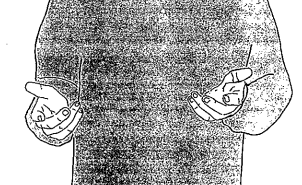
\includegraphics[width=5cm]{figures/heresmypoint}
\caption{\enquote{Here's my point.}}
\label{fig:mypoint}
\end{figure}


The \enquote*{open hand} pointing gesture in Figure~\ref{fig:yourturn} acts as a turn-taking device: it can function as a \isi{turn-assigning gesture} (underlined by the caption of Figure~\ref{fig:yourturn}), or, when used to point at the current speaker, it can also indicate that the gesturer wants to take the turn and address the current turn holder.

\begin{figure}
  \centering
  % \includegraphics[trim={11cm 4cm 13cm 10.5cm}, clip, angle=90, width=5cm]{figures/InteractiveGestures}
  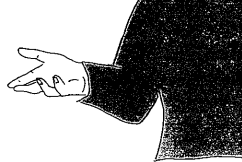
\includegraphics[width=4.5cm]{figures/goahead}
\caption{\enquote{You go ahead.}}
\label{fig:yourturn}
\end{figure}

So far there is no account of interactive gestures in HPSG. 
%
Given their entrenchment in dialogue processes, their natural home seems to be in a dialogue theory, anyway (see \crossrefchapteralt{pragmatics}).
%
Accordingly, what is presumably the only formal approach to some of these gestures has been spelled out within the dialogical framework PTT in \citet{Rieser:Poesio:2009}.
\is{interactive gestures|)}




\section{Gesture and \ldots}
\label{sec:gesture-and}

Besides being of a genuine linguistic, theoretical interest, gesture studies are a common topic in various areas of investigation, some of which are briefly pointed at below. 


\subsection{\ldots\ tools, annotation, corpora}
\label{sec:tools-annotation-corpora}

Since gestures are signs in the visual modality, they have to be videotaped.
%
Gesture annotation is carried out on the recorded video films.
%
The main tools that allow for video annotation are, in alphabetical order, \isi{Anvil}\footnote{%
\url{https://www.anvil-software.org/}, \citealp{Kipp:2014}.
}, \isi{ELAN}\footnote{%
\url{https://tla.mpi.nl/tools/tla-tools/elan/}, Max Planck Institute for Psycholinguistics, The
Language Archive, Nijmegen, The Netherlands, \citealp{Sloetjes:Wittenburg:2008}.}
and \isi{EXMARaLDA}\footnote{%
\url{https://exmaralda.org/}, \citealp{Schmidt:2012}.
}.

Annotation should follow an annotation standard which is specified in an annotation scheme.
%
Various annotation schemes for gestures and speech-gesture integration have been proposed, partly differing in annotation foci, including the following ones:
%
annotation schemes that focus on form description and gestures classification in terms of a taxonomy like the one introduced in Section~\ref{sec:kinds-gestures} have been developed by R. Breckenridge Church, published in the appendix of \citet{McNeill:1992}; CoGEST \citep{Gibbon:et:al:2003}; FORM \citep{Martell:Osborn:Friedman:Howard:2002} and the SaGA annotation \citep{Luecking:Bergmann:Hahn:Kopp:Rieser:2013}.
%
The form of gestures and their timing with speech is the object of the coding scheme of \citet{Kipp:Neff:Albrecht:2007}.
%
An interaction-oriented scheme has been proposed by \citet{Allwood:et:al:2007}, which is formulated on the level of turns and dialogue management.
%
A detailed annotation scheme for the form and function of gestures has been developed in terms of \enquote{annotation decision trees} within the NEUROGES system \citep{Lausberg:Sloetjes:2009}.


Annotated videos of real life interactions give rise to multimodal corpora. 
%
Among those that include data on gestures are the following ones.

The multimodal \isi{SmartKom Corpus} \citep{Schiel:Steininger:Tuerk:2003}, which grew out of the SmartKom project \citep{Wahlster:2006}, comprises recording sessions of various Wizard-of-Oz experiments (that is, human-computer interaction where the human participant is made to believe that the system she or he interacts with is autonomous while in fact it is, at least partly, operated by another human).
%
Recordings are extended basically by a transliteration and labelling of natural speech, labelling of gestures and annotation of user states (in the corpus' first release). 
%
The first public release, SKP 1.0, contains 90 recording sessions of 45 users. 
%
The multimodal SmartKom corpus as well as further SmartKom resources are hosted at the \textit{\ili{Bavarian} Archive for Speech Signals} (\url{https://www.bas.uni-muenchen.de/Bas/}).


The \isi{AMI Meeting Corpus} \citep{Carletta:et:al:2006} consists of 100 hours of meeting recordings.
%
The meetings were recorded in \ili{English} but include mostly non-native speakers. 
%
The AMI Meeting Corpus provides orthographic transcriptions, but also has a couple of further annotations, including dialogue acts, named entities, head gesture, hand gesture, gaze direction, movement and emotional states.


The SaGA (\enquote{Speech and Gesture Alignment}) corpus \is{SaGA Corpus} consists of 24 \ili{German} route direction dialogues obtained after a bus ride through a virtual town \citep{Luecking:Bergmann:Hahn:Kopp:Rieser:2010}. 
%
Audio and video data from the direction-giver were recorded. 
%
The SaGA corpus consists of 280 minutes of video material containing 4,961 iconic/deictic gestures, approximately 1,000 discourse gestures and 39,435 word tokens \citep{Luecking:Bergmann:Hahn:Kopp:Rieser:2013}.
%
Gesture annotation has been carried out in great detail, following a kinematic, form-based approach (cf. the above-given remark on annotation schemes).
%
Part of the SaGA corpus is available from the \textit{\ili{Bavarian} Archive for Speech Signals} (\url{https://www.bas.uni-muenchen.de/Bas}).


The DUEL (\enquote{Disfluency, exclamations and laughter in dialogue}) corpus \is{DUEL Corpus} \citep{Hough:Tian:de:Ruiter:Betz:Kousidis:Schlangen:Ginzburg:2016} comprises 24 hours of natural, face-to-face dialogue in \ili{German}, \ili{French} and \ili{Mandarin Chinese}.
%
It includes audio, video and body tracking data and is transcribed and annotated for disfluency, laughter and exclamations.


The FIGURE (derived from \enquote{Frankfurt Image GestURE}) corpus \is{FIGURE Corpus} \citep{Luecking:Mehler:Walther:Mauri:Kurfuerst:2016} is built on recordings of 50 participants with various mother tongues (though mostly \ili{German}) spontaneously producing gestures in response to five or six terms from a total of 27 stimulus terms, which have been compiled mainly from image schemata \citep{Lakoff87a-u}.
%
The gestures have been kinematically annotated by means of a variant of the SaGA annotation scheme.
%
The FIGURE annotation is available from the Text Technology Lab Frankfurt (\url{https://www.texttechnologylab.org/applications/corpora}).



\subsection{\ldots\ robots and virtual agents}
\label{sec:virtual-agents}

In the context of Human-Computer Interaction (HCI) or Human-Robot Interaction (HRI), gesture plays an important role (in fact, the formal modelling of deictic and iconic gestures has been initiated in these fields, cf. Section~\ref{sec:precursors}).
%
One reason for this prominence of gesture in technical areas is that people who interact with a robot evaluate it more positively when the robot displays non-verbal behaviours such as hand and arm gestures along with speech (see e.g.\ \citealt{Salem:et:al:2012}).
%
Within HCI/HRI, two kinds of distinctions have to be made. 
%
The first is a distinction between \enquote{robot} in the sense of virtual avatars and \enquote{robot} in the (probably more common) sense of physical devices (only the latter will be henceforth called a \enquote{robot}).
%
The second distinction discerns gesture generation from gesture recognition.
%
Given this simple systematization, altogether four divisions of gesture and virtual avatars/robots arise (references are just exemplary and preferably from earlier HCI/HRI times):
%
(i) gesture generation by robots \citep[e.g.][]{Le:et:al:2011};
%
(ii) gesture recognition by robots \citep[e.g.][]{Triesch:vanDerMalsburg:1998};
%
(iii) gesture generation by virtual avatars \citep[e.g.][]{Cassell:Stone:Yan:2000};
%
and (iv) gesture recognition in VR/AR \citep[e.g.][]{Weissmann:Salomon:1999}.
%
For a more detailed overview see \citet{Luecking:Pfeiffer:2012}.
%
Enabling humans to act and interact in virtual rooms \citep[e.g.][]{Pfeiffer:et:al:2018} can be seen as recent extension of gesture use in HCI/HRI.


In order to plan and design the speech/gesture output of a virtual avatar or a robot, a multimodal representation format is required.
%
To this end, the \textit{Multimodal Utterances Representation Markup Language} for conversational robots (MURML) has been developed \citep{Kranstedt:Kopp:Wachsmuth:2002:b}.
%
A similar purpose is served by the \textit{Extensible MultiModal Annotation} \citep[EMMA;][]{Johnston:2009}.





\subsection{\ldots\ learning}
\label{sec:learning}

Following a \enquote{gesture as a window to the mind} view, gestures must be a prime object of educational theory and practice, and they are indeed, as demonstrated by research of \citet{Cook:Goldin-Meadow:2006} and colleagues.
%
Effectiveness of gestures has been studied in math lessons \citep{Goldin-Meadow:Nusbaum:Kelly:Wagner:2001}, in the acquisition of counting competence \citep{Alibali:DiRusso:1999} and in bilingual education \citep{Breckinridge-Church:Ayman-Nolley:Mahootian:2004}, among other areas.
%
The fairly unanimous result is that gestures can indeed reflect students' conceptualisations and provide insights into cognitive processes involved in learning.
%
Therefore, they can be used as a teaching device as well as an indicator of learning progress and understanding. 



\subsection{\ldots\ aphasia}
\label{sec:aphasia}

Current models of utterance production are speech-gesture production models, assuming a (more or less) integrated generation of multimodal utterances.
%
Based on such models, one expects an effect on gesture performance when speech production is impaired, as is the case with aphasic speakers. 
%
Aphasia \is{aphasia} is an acquired speech disorder, which can be caused by a stroke, ischaemia, haemorrhage, craniocerebral trauma and further brain-damaging diseases.
%
Different speech-gesture production models make slightly different predictions for speakers suffering from aphasia and can be evaluated accordingly \citep{deRuiter:deBeer:2013}.
%
Indeed, observing the gesture behaviour of aphasic speakers is one aspect of gesture and aphasia \citep{Jakob:Bartmann:Goldenberg:Ziegler:Hogrefe:2011,Kong:Law:Chak:2017,Sekine:Rose:2013}.
%
\is{speech-gesture production models|(}
With the exception of the growth point theory, speech-gesture production models are based on Levelt's (\citeyear{Levelt:1989}) \ia{Levelt} model.

The \emph{Growth Point model} \citep{McNeill:Duncan:2000} assumes that the \enquote{seed} of an utterance is an inherently multimodal idea unit that comprises imagistic as well as symbolic proto-representations which unfold into gesture and speech respectively in the process of articulation \citetext{see also \citealt{Roepke:2011} on the growth point's entrenchment in contexts and frames}.

The \emph{Sketch model} \is{sketch model} \citep{de:Ruiter:2000} reflects explicitly different kinds of gestures (see Section~\ref{sec:kinds-gestures}). 
%
Its name is due to the sketch component, an abstract spatio-temporal representation alongside Levelt's preverbal message. 
%
Independently from each other, the sketch is sent to a gesture planner, while the preverbal message is processed by the formulator.

According to the \emph{Lexical Access model} \is{Lexical Access model} of \citet{Krauss:Chen:Gottesmann:2000}, iconic gestures are related to words and are used in order to facilitate speaker-internal word retrieval rather than communicating pictorial information.

The \emph{Interface model} \is{Interface model} \citep{Kita:Ozyurek:2003} assumes that the processes for speech and gesture generation negotiate with each other and therefore can influence each other during the production phase.
\is{speech-gesture production models|)}

Other aspects include the use of gesture in speech therapy. 
%
Very much in line with the lexical access model, gestures have been used in order to facilitate word retrieval in what can be called \emph{multimodal therapy} \is{multimodal therapy} \citep{Rose:2006}.
%
Following a different strategy, gestures are also used in order to enhance the communicative range of patients: they learn to employ gestures instead of words in order to communicate at least some of their needs and thoughts more fluently \citep{Cubelli:Trentini:Montagna:1991,Caute:et:al:2013}.

However, just counting on gestures in therapy does not automatically lead to success \citep{Auer:Bauer:2011}. 
%
The type and severity of aphasia, the individual traits of the aphasic speaker and the kinds of gestures impaired or still at disposal, among other factors, seem to constitute a complex network for which currently no generally applicable clinical pathway can be given.




\section{Outlook}
\label{sec:outlook}

What are (still) challenging issues with respect to grammar-gesture integration, in particular from a semantic point of view? Candidates include:

\begin{itemize}
\item gestalt phenomena: the trajectories described by a gesture are often incomplete and have to be completed by drawing on gestalt principles or everyday knowledge \citep{Luecking:2016}.
%%
\item negligible features: not all formal features of a gesture are meaning"=carrying features in the context of utterance. For instance, in a dynamic gesture the handshape often (though not always) does not provide any semantic information (cf. also examples (\ref{ex:half-circle-gesture}) and (\ref{ex:mud-rmrs})/Figure~\ref{fig:interpret-circular})). How can we distinguish between significant and negligible gesture features?
%%
\item \enquote{semantic endurance}: due to holds, gestures can show their meaning contributions for some period of time and keeps available for semantic attachment. This may call for a more sophisticated algebraic treatment of speech-gesture integration than offered by typed feature structures \citep{Rieser:2015}.
\end{itemize}

Finally, the empirical domain of \enquote{gesture} has to be extended to other non-verbal signals, in particular propositional ones such as laughter \citep{Ginzburg:Breitholz:Cooper:Hough:Tian:2015}, facial expressions or gaze (see Section~\ref{sec:why-gestures} for a brief list of non-verbal signals), in isolation as well as in mutual combination.
%
Thus, there is still some way to go in order to achieve a fuller understanding of natural language interaction and thereby natural languages.


 
% \section*{Abbreviations}
\section*{Acknowledgements}


This work is partially supported by a public grant overseen by the \ili{French} National Research Agency (ANR) as part of the program ``Investissements d'Avenir'' (reference: ANR-10-LABX-0083). It contributes to the IdEx Université de Paris -- ANR-18-IDEX-0001. For insightful comments on earlier drafts I want to thank Anne Abeillé, Jonathan Ginzburg, Alex Lascarides, Stefan Müller, Hannes Rieser, and Markus Steinbach. They helped to improve the chapter a lot. Needless to say that all remaining oddities or shortcomings are my own. Furthermore, I am grateful to Elizabeth Pankratz for attentive remarks and for proofreading. 



{\sloppy
\printbibliography[heading=subbibliography,notkeyword=this]
}
\end{document}






